%%%
%%% iTrameRA : Trame pour le Rapport d'Activité Inria 2016
%%% ------------------------------------------------------
%%% 
%%% Url de la trame : http://irabot.inria.fr/itramera?projet=eva
%%%
%%% ----------------
%%%  Nouveautés 2016 !
%%% ----------------
%%% 
%%% - Mots-clés : une application dédiée à mettre à jour et un import dans le RA
%%% - Logiciels : à renseigner dans Bil avant l'import dans le RA
%%% ------------------
%%% Ce document est un squelette de rapport d'activité 
%%% mis à jour à partir des bases de données de l'Inria
%%% (HAL pour les publis, BASTRI pour les équipes, Bil pour les logiciels, l'entrepôt pour les données DPEI ...).
%%% Le rédacteur doit compléter ce document. 
%%%
%%% Marche à suivre :
%%%
%%% Récuperer l'archive tgz de 2016 et la décompresser  dans un répertoire. 
%%% Il y a un fichier tex et 3 fichiers de bibliographie (.bib) : 
%%% - eva2016.tex : le texte en latex du rapport 
%%% - eva2016.bib : les publis de l'année 2016 issues de Hal
%%% - eva_refer2016.bib : les publications de référence (c'est-a-dire les publis les plus importantes
%%%   de l'équipe quelle que soit l'année)
%%% - eva_foot2016.bib : les publis placées dans les notes de bas de page (footnote) issues de votre rapport 2015
%%%
%%% Instructions pour l'écriture du RA :
%%%
%%% https://intranet.inria.fr/Vie-scientifique/Information-edition-scientifiques/Comment-rediger-le-RAweb/Rediger-le-RA-Objectifs-et-actualites
%%%
%%% Pour compiler puis déposer le rapport utiliser le serveur iRAbot : 
%%%
%%% http://irabot.inria.fr/irabot
%%%
%%% ou bien le script irabot.sh qui utilise iRAbot.
%%% Certains centres ont leur propre serveur de compilation.
%%%
%%% Le rapport est en ANGLAIS !
%%%

\documentclass{ra2016}

%SKEL - v0.4 - 2016 (Utiliser pour les stats d'utilisation de Skel, merci de ne effacer cette ligne)

% ne pas enlever 
\renewenvironment{motscle}{\begin{xmlelement}{keywords}}{\end{xmlelement}}

%%% Par defaut sont inclus les packages : html, french, graphics et footbib 
%%% (ifthen curves soul epsf html)
%%% Le plus souvent la commande \usepackage n'est pas prise en compte 
%%% Mais si le package est calc ou fp certaines commandes sont rendues disponibles
%%% (fancyvrb) 

%%% Mettez ici les \newcommand et \def que vous voulez

%%%%%%%%%%%%%%%%%%%%%%%%%%%%%%%%%%%%%%%%%%%%%%%%%%%%%%%%%%%%%%%%%%%%%%%%%%%%%%
% Fonctions tex issus du RAweb 2015
% Source : eva2015.tex
% Date : jeudi 17 novembre 2016, 10:40:56 (UTC+0100)
%

\newcommand{\paul}             {\textbf{Paul~Muhlethaler}}
\newcommand{\pascale}          {\textbf{Pascale~Minet}}
\newcommand{\thomas}           {\textbf{Thomas~Watteyne}}
\newcommand{\achir}            {\textbf{Nadjib~Achir}}

\newcommand{\commentthomas}[1] {\textbf{[Thomas] #1}}

%%%%%%%%%%%%%%%%%%%%%%%%%%%%%%%%%%%%%%%%%%%%%%%%%%%%%%%%%%%%%%%%%%%%%%%%%%%%%%
%%%
%%%  Information sur les données importées : Bastri
%%%
%%% Les organismes ou écoles partenaires de votre équipe ainsi que les labos auxquels
%%% vous êtes associés seront affichés automatiquement et à postériori, comme vos CRI, 
%%% thème et domaine de rattachement. Ces infos sont issues de Bastri : 
%%% https://bastri.inria.fr, la base des structures de recherche Inria.
%%%
%%% L'acronyme de votre équipe sera également présenté comme dans les fiches projets.
%%% Si vous souhaitez le modifier, faites-le dans la base de gestion des fiches projets :
%%% https://bastri.inria.fr/FichesProjets/ et régénérez votre trame.
%%%
%%% Le "moreinfo" de l'équipe servira donc uniquement à préciser la localisation 
%%% quand elle est distincte du CRI (pour ceux qui le souhaitent).  
%%% 
%%% Vérifiez et signalez erreurs et problèmes : raweb-support@inria.fr
%%%
%%%%%%%%%%%%%%%%%%%%%%%%%%%%%%%%%%%%%%%%%%%%%%%%%%%%%%%%%%%%%%%%%%%%%%%%%%%%%%

%%% \projet{<PROJET>}{<ALT-ABRÉGÉ>}{<NOM-PROJET-EXPLICITÉ>}
%%% exemple : 
%%% \projet{EXEMPLE}{ExemplE}{Algebraic Systems for Research and Industry} 
%%%

%%%%%%%%%%%%%%%%%%%%%%%%%%%%%%%%%%%%%%%%%%%%%%%%%%%%%%%%%%%%%%%%%%%%%%%%%%
% Informations concernant l'equipe extraites de BASTRI
% Source : http://bastri.inria.fr/
% Date : jeudi 17 novembre 2016, 10:40:56 (UTC+0100)
%

\projet{EVA}{eva}{Wireless Networking for Evolving \& Adaptive Applications}

%% Pour information le domaine et le theme du projet 
%% Domaine : Networks, Systems and Services, Distributed Computing
%% Theme : Networks and Telecommunications

%%% CRI Inria 
%%% Sophia, ou Paris, ou Nancy, si le projet est bilocalisé : \UR{cr1,cr2} etc

\UR{Paris}

%%% Cartographie de l'activité : chaque équipe aura à renseigner les mots-clés 2016 décrivant son activité sur une application dédiée.  
%%% Le RA les importera dans la trame. Cet import pourra se faire juste avant la mise en ligne sur Inria.fr (non disponible lors des phases de rédaction).
%%% https://intranet.inria.fr/Vie-scientifique/Information-edition-scientifiques/Comment-rediger-le-RAweb/Consignes-generales#eztoc26917_3

%%%%%%%%%%%%%%%%%%%%%%%%%%%%%%

\begin{document}
\maketitle

%%% Attention, il n'y a pas de \nocite{*} implicite. 
%%% Une commande \nocite{*} a été ajoutée.
%%% Vous pouvez utiliser des \nocite{xx}.

%\nocite{TFE98}
%\nocite{AGATHISC}
%\nocite{FD98}
%\nocite{x,y,z} 

%%% Pour ceux qui le souhaitent le moreinfo permet d'insérer un texte
%%% de 3 - 4 lignes qui indique les particularités de l'équipe
%%% Il permet par exemple de préciser la localisation quand elle est distincte du CRI. 
%%% Ne doublonnez pas thème, domaine, CRI et partenariats qui sont ajoutés automatiquement. 

\begin{moreinfo}
%%ICI Vous pouvez ecrire du texte
\end{moreinfo}

%%%%%%%%%%%%%%%%%%%%%%%%%%%%%%%%%%%%%%%%%%%%%%%%%%%%
%%%
%%% Liste des modules possibles pour les sections :
%%% presentation* fondements domaine logiciels
%%% resultats contrats* partenariat* diffusion*
%%%
%%% ex : \begin{module}{composition}
%%%
%%% \begin{module} {<SECTION>} {<NOMMODULE>} {<TITRE>}
%%%     <PERSONNES> 
%%%    [<GLOSSAIRE>] 
%%%    [<MOREINFO>] 
%%%    [<RESUME>]  
%%%    <CORPS>
%%% \end{module}
%%%
%%%
%%% NOMMODULE est un identifiant unique pour reperer le module,
%%% aussi chaque module doit en avoir un NOMMODULE different  
%%%
%%% \begin{module}{logiciels}{calcul-formel}{Sofrware aspects of Computer Algebra}
%%%  \begin{participants}
%%%  format: \pers <PRENOM> [<PARTICULE>] <NOM> [<MOREINFO>]
%%%        \pers{Jean}[de]{La Fontaine}[1621-1695],
%%%        \pers{Cecil Blount}{De Mille}
%%%  \end{participants}
%%%  \begin{glossaire}
%%%       \glo{backward combatability}{A property of hardware or software
%%%   ... but activeliy... }
%%%  \end{glossaire}
%%%  \begin{abstract}
%%%       Le joli résumé que voilà
%%%  \end{abstact} 
%%%  This is a very short module with a hypertext link to the
%%%  \href{http://www.eps.mcgill.ca/jargon/jargon.html}{Jargon File}.
%%% \end{module}
%%%
%%%%%%%%%%%%%%%%%%%%%%%%%%%%%%%%%%%%%%%%%%%%%%%%%%%%%%%%%%%%%%%%%%%%%

%%%%%%%%%%%%%%%%%%%%%%%%%%%%%%%%%%%%%%%%%%%%%%%%%%%%%%%%%%%%%%%%%%%%%
%%%
%%% Composition de l'equipe
%%%
%%% Professions possibles :
%%% Visiteur Chercheur Enseignant Technique Assistant
%%% PhD PostDoc AutreCategorie
%%% 
%%% Utiliser le mot-clé [Habilite] pour les titulaires d'une Thèse d'État ou d'une HDR
%%%
%%%       \pers{Prénom}{Nom}{profession}[champ_libre: Employeur, Fonction, until/since, financement, info supplémentaire][Habilite]?
%%%        ...
%%%
%%% La mention "Team leader" est précisée dans le champ libre (moreinfo) et pré-remplie par l'export GEF.
%%%
%%% Dans le champ libre, si vous indiquez le grade (donnée importée si elle est dans Gef), écrivez :
%%%    
%%%   Pour DR : Senior Researcher 
%%%   Pour CR : Researcher
%%%   Pour Advanced Research position : Advanced Research position
%%%   Pour Starting Research position : Starting Research position
%%%   Pour Professeur : Professor ou Prof
%%%   Pour Maitre de conférence : Associate Professor

%%%
%%%%%%%%%%%%%%%%%%%%%%%%%%%%%%%%%%%%%%%%

%%%%%%%%%%%%%%%%%%%%%%%%%%%%%%%%%%%%%%%%%%%%%%%%%%%%%%%%%%%%%%%%%%%%%%
%%%
%%% Information sur les données importées : membres de l'équipe
%%% 
%%% Les membres permanents et ceux connus de la DRH sont exportés de GEF, base DRH.
%%% Les infos de financement viennent de la base OSC des contrats et la graphie des noms des responsables d'équipe de Bastri.
%%% Vérifier si les noms sonts corrects 
%%% La mention "Team leader" est exportée dans le champ libre (moreinfo), de même que l'employeur (à vérifier)
%%% Vérifiez et signalez erreurs et problèmes : raweb-support@inria.fr 
%%%
%%%%%%%%%%%%%%%%%%%%%%%%%%%%%%%%%%%%%%%%%%%%%%%%%%%%%%%%%%%%%%%%%%%%%% 

 %%% https://intranet.inria.fr/Vie-scientifique/Information-edition-scientifiques/Comment-rediger-le-RAweb/Les-sections#eztoc27554_2
 %%% L'exemple ne s'applique pas aux projets multi-localisés, qui ajouteront le CRI de rattachement après chaque nom entre [].

%%%%%%%%%%%%%%%%%%%%%%%%%%%%%%%%%%%%%%%%%%%%%%%%%%%%%%%%%%%%%%%%%%%%%%%%%%%%%%
% Donnees  construites d'après les informations de la base GEF pour 2016
% Source : https://gef.inria.fr/
% Date : jeudi 17 novembre 2016, 10:40:56 (UTC+0100)
%

\begin{composition}
    % Research Scientists (Chercheur)
    \pers{Pascale}{Minet}{Chercheur}[Inria, Research Scientist][Habilite]
    \pers{Paul}{Muhlethaler}{Chercheur}[Inria, Team leader, Research Scientist][Habilite]
    \pers{Thomas}{Watteyne}{Chercheur}[Inria, Research Scientist]
    % Engineers (Technique)
    \pers{Tengfei}{Chang}{Technique}[Inria, Postdoctoral Research Engineer]
    \pers{Ines}{Khoufi}{Technique}[Inria, Postdoctoral Research Engineer]
    \pers{R\'emy}{Leone}{Technique}[Inria, Postdoctoral Research Engineer, started Feb 2016]
    \pers{Erwan}{Livolant}{Technique}[Inria, Research Engineers, until Nov 2016]
    \pers{Malisa}{Vucinic}{Technique}[Inria, Postdoctoral Research Lead, started Sep 2016]
    % PhD students (PhD)
    \pers{Nesrine}{Ben Hassine}{PhD}[Inria, PhD Student]
    \pers{Younes}{Bouchaala}{PhD}[Vedecom, PhD Student]
    \pers{Keoma}{Brun-Laguna}{PhD}[Inria, PhD Student]
    \pers{Mohamed}{Elhadad}{PhD}[ATER Paris V, PhD Student]
    \pers{Fatma}{Marzouk}{PhD}[Ensi, PhD Student]
    \pers{Jonathan}{Mu\~noz}{PhD}[Gridbe, PhD Student, CIFRE]
    % Post-Doctoral Fellow (PostDoc)
    \pers{Ehsan}{Ebrahimi Khaleghi}{PostDoc}[Inria, Post-Doctoral Fellow, started May 2016]
    % Visiting Scientists (Visiteur)
    \pers{Mario}{Gerla}{Visiteur}[    Professor,   UCLA,                       USA,    visit 10-20 December 2016]
    \pers{Felipe}{Lalanne}{Visiteur}[ Reseacher,   Inria Chile,                Chile,  visit 19–26 Octobre 2016]
    \pers{Mario}{Gerla}{Visiteur}[    Professor,   UCLA,                       USA,    visit 31 August - 23 September 2016]
    \pers{Travis}{Massey}{Visiteur}[  PhD Studen,  UC Berkeley,                USA,    visit 22 July 2016]
    \pers{Diego}{Dujovne}{Visiteur}[  Professor,   Universidad Diego Portales, Chile,  visit 22-31 July 2016]
    \pers{Carlos}{Oroza}{Visiteur}[   PhD Student, UC Berkeley,                USA,    visit 23-29 July 2016]
    \pers{David}{Burnett}{Visiteur}[  PhD Student, UC Berkeley,                USA,    visit 13-15 June 2016]
    \pers{Branko}{Kerkez}{Visiteur}[  Professor,   U. Michigan,                USA,    visit 17-22 June 2016]
    \pers{Steven}{Glaser}{Visiteur}[  Professor,   UC Berkeley,                USA,    visit 21-25 March 2016]
    \pers{Filip}{Barac}{Visiteur}[    PhD Student, Mid Sweden University,      Sweden, visit 8-19 February 2016]
    \pers{Xavi}{Vilajosana}{Visiteur}[Professor,   UOC/OpenMote,               Spain,  visit 2-4 February 2016]
    % Administrative Assistant (Assistant)
    \pers{Christine}{Anocq}{Assistant}[Inria, Assistant]
    % Others (AutreCategorie)
    \pers{Nadjib}{Achir}{AutreCategorie}[Univ. Paris XIII, Associate Professor][Habilite]
    \pers{Selma}{Boumerdassi}{AutreCategorie}[CNAM,  Associate Professor]
    \pers{Samia}{Bouzefrane}{AutreCategorie}[CNAM, Associate Professor]
    \pers{Philippe}{Jacquet}{AutreCategorie}[Bell Labs (Alcatel), Division Leader][Habilite]
    \pers{Anis}{Laouiti}{AutreCategorie}[France Telecom, Associate Professor][Habilite]
    \pers{Dana}{Marinca}{AutreCategorie}[Univ. Versailles,Associate Professor]
    \pers{Nadjib}{Ait Saadi}{AutreCategorie}[Univ. Paris Est, Associate Professor]
    \pers{Jiangnan}{Yang}{AutreCategorie}[Inria, Internship, Apr-Aug 2016]
\end{composition}

%%%%%%%%%%%%%%%%%%%%%%%%%%%%%%%%%%%%%%%%%%%%%%%%%%%%%%%%%%%%%%%%%%%%%%%%%%
%%%
%%% Section presentation (Overall Objectives)
%%% On peut mettre un ou plusieurs modules.
%%% 
%%% La partie présentation du projet est issue de la section "Overall Objectives" du RAweb 2015 
%%% source : http://raweb.inria.fr/rapportsactivite/2015/eva/uid0.html
%%%
%%%%%%%%%%%%%%%%%%%%%%%%%%%%%%%%%%%%%%%%%%%%%%%%%%%%%%%%%%%%%%%%%%%%%%%%%%

%%% https://intranet.inria.fr/Vie-scientifique/Information-edition-scientifiques/Comment-rediger-le-RAweb/Les-sections#eztoc27554_5

%%%%%%%%%%%%%%%%%%%%%%%%%%%%%%%%%%%%%%%%%%%%%%%%%%%%%%%%%%%%%%%%%%%%%%%%%%%%%%
% Présentation du projet issues des informations du RAweb 2015
% Source : http://raweb.inria.fr/rapportsactivite/RA2015/eva/uid3.html
% Date : jeudi 17 novembre 2016, 10:40:56 (UTC+0100)
%

%==============================================================================
\begin{module}{presentation}{overall-objectives}{Overall Objectives}

It is forecast that the vast majority of Internet connections will be wireless.
The EVA project grasps this opportunity and focus on wireless communication.
EVA tackles challenges related to providing efficient communication in wireless networks and, more generally, in all networks that are not already organized when set up, and consequently need to evolve and spontaneously find a match between application requirements and the environment.
These networks can use opportunistic and/or collaborative communication schemes.
They can evolve through optimization and self-learning techniques.
Every effort is made to ensure that the results provided by EVA have the greatest possible impact through standardization.
The miniaturization and ubiquitous nature of computing devices has opened the way to the deployment of a new generation of wireless (sensor) networks.
These networks are central to the work in EVA, as EVA focuses on such crucial issues as power conservation, connectivity, determinism, reliability and latency.
Wireless Sensor Network (WSN) deployments are also be a new key subject, especially for emergency situations (e.g.~after a disaster).
Industrial process automation and environmental monitoring are considered in greater depth.

\end{module}

%%%%%%%%%%%%%%%%%%%%%%%%%%%%%%%%%%%%%%%%%%%%%%%%%%%%%%%%%%%%%%%%%%%%%%%%%%%%%
%%%
%%% Module fondements (Research Program)
%%%
%%% Ce module fondements va apparaitre dans le rapport en html et en pdf sous le titre "Research Program",
%%% anciennement le titre était "Scientific Foundations" mais le contenu reste le même. 
%%%
%%% Cette section sert à mentionner le contexte scientifique qui est à la base de votre programme 
%%% puis à préciser les différentes thématiques que vous abordez au sein de votre équipe-projet. 
%%%
%%%%%%%%%%%%%%%%%%%%%%%%%%%%%%%%%%%%%%%%%%%%%%%%%%%%%%%%%%%%%%%%%%%%%%%%%%%%%

%==============================================================================
\begin{module}{fondements}{test1}{Generalities}

EVA inherits its expertise in designing  algorithms and protocols from HiPERCOM2 (e.g. OLSR).
EVA also inherit know-how in modeling, simulation, experimentation and standardization.
Through this know-how and experience, the results obtained are both far-reaching and useful.

\end{module}

%==============================================================================
\begin{module}{fondements}{sec:phylayer}{Physical Layer}

We plan to study how advanced physical layers can be used in low-power wireless networks.
For instance, collaborative techniques such as multiple antennas (e.g. the Massive MIMO technology) can improve communication efficiency.   
The idea is to use a massive network densification by drastically increasing the number of sensors in a given area in a Time Division Duplex (TDD) mode with time reversal.
The first period allows the sensors to estimate the channel state and, after time reversal, the second period is to transmit the data sensed.
Other techniques, such as interference cancellation, are also possible.

\end{module}

%==============================================================================
\begin{module}{fondements}{sec:wirelessaccess}{Wireless Access}

Medium sharing in wireless systems has received substantial attention throughout the last decade.
HiPERCOM2 has provided models to compare TDMA and CSMA.
HiPERCOM2 has also studied how network nodes must be positioned to optimize the global throughput.

EVA will pursue modeling tasks to compare access protocols, including multi-carrier access, adaptive CSMA (particularly in VANETs), as well as directional and multiple antennas.
There is a strong need for determinism in industrial networks.
The EVA team will focus particularly on scheduled medium access in the context of deterministic industrial networks; this will involve optimizing the joint time slot and channel assignment.
Distributed approaches will be considered, and the EVA team will determine their limits in terms of reliability, latency and throughput.
Furthermore, adaptivity to application or environment changes will be taken into account.

\end{module}

%==============================================================================
\begin{module}{fondements}{sec:coex}{Coexistence of Wireless Technologies}

Wireless technologies such as cellular, low-power mesh networks, (Low-Power) WiFi, and Bluetooth (low-energy) can reasonably claim to fit the requirements of the IoT.
Each, however, uses different trade-offs between reliability, energy consumption and throughput.
The EVA team will study the limits of each technology, and will develop clear criteria to evaluate which technology is best suited to a particular set of constraints.

Coexistence between these different technologies (or different deployments of the same technology in a common radio space) is a valid point of concern.

The EVA team aims at studying such coexistence, and, where necessary, propose techniques to improve it.
Where applicable, the techniques will be put forward for standardization.
Multiple technologies can also function in a symbiotic way.

For example, to improve the quality of experience provided to end users, a wireless mesh network can transport sensor and actuator data in place of a cellular network, when and where cellular connectivity is poor.

The EVA team will study how and when different technologies can complement one another.
A specific example of a collaborative approach is Cognitive Radio Sensor Networks (CRSN).

\end{module}

%==============================================================================
\begin{module}{fondements}{sec:enereff}{Energy-Efficiency and Determinism}

Reducing the energy consumption of low-power wireless devices remains a challenging task.
The overall energy budget of a system can be reduced by using less power-hungry chips, and significant research is being done in that direction. 
Nevertheless, power consumption is mostly influenced by the algorithms and protocols used in low-power wireless devices, since they influence the duty-cycle of the radio.

EVA will search for energy-efficient mechanisms in low-power wireless networks.
One new requirement concerns the ability to predict energy consumption with a high degree of accuracy.
Scheduled communication, such as the one used in the IEEE 802.15.4e TSCH (Time Slotted CHannel Hopping) standard, and by IETF 6TiSCH, allows for a very accurate prediction of the energy consumption of a chip. Power conservation will be a key issue in EVA.

To tackle this issue and match link-layer resources to application needs, EVA's 5-year research program around Energy-Efficiency and Determinism centers around 3 studies:

\begin{itemize}
    \item Performance Bounds of a TSCH network.
        We propose to study a low-power wireless TSCH network as a Networked Control System (NCS), and use results from the NCS literature.
        A large number of publications on NCS, although dealing with wireless systems, consider wireless links to have perfect reliability, and do not consider packet loss.
        Results from these papers can not therefore be applied directly to TSCH networks.
        Instead of following a purely mathematical approach to model the network, we propose to use a non-conventional approach and build an empirical model of a TSCH network.
    \item Distributed Scheduling in TSCH networks.
       Distributed scheduling is attractive due to its scalability and reactivity, but might result in a sub-optimal schedule.
       We continue this research by designing a distributed solution based on control theory, and verify how this solution can satisfy service level agreements in a dynamic environment.
\end{itemize}

\end{module}

%==============================================================================
\begin{module}{fondements}{sec:netdep}{Network Deployment}

Since sensor networks are very often built to monitor geographical areas, sensor deployment is a key issue.
The deployment of the network must ensure full/partial, permanent/intermittent coverage and connectivity.
This technical issue leads to geometrical problems which are unusual in the networking domain.

We can identify two scenarios.
In the first one, sensors are deployed over a given area to guarantee full coverage and connectivity, while minimizing the number of sensor nodes.
In the second one, a network is re-deployed to improve its performance, possibly by increasing the number of points of interest covered, and by ensuring connectivity.
EVA will investigate these two scenarios, as well as centralized and distributed approaches.
The work starts with simple 2D models and will be enriched to take into account more realistic environment: obstacles, walls, 3D, fading. 

\end{module}

%==============================================================================
\begin{module}{fondements}{sec:datgath}{Data Gathering and Dissemination}

A large number of WSN applications mostly do data gathering (a.k.a ``convergecast'').
These applications usually require small delays for the data to reach the gateway node, requiring time consistency across gathered data.
This time consistency is usually achieved by a short gathering period.

In many real WSN deployments, the channel used by the WSN usually encounters perturbations such as jamming, external interferences or noise caused by external sources (e.g.~a polluting source such as a radar) or other coexisting wireless networks (e.g.~WiFi, Bluetooth).
Commercial sensor nodes can communicate on multiple frequencies as specified in the IEEE 802.15.4 standard.
This reality has given birth to the multichannel communication paradigm in WSNs.

Multichannel WSNs significantly expand the capability of single-channel WSNs by allowing parallel transmissions, and avoiding congestion on channels or performance degradation caused by interfering devices.

In EVA, we will focus on raw data convergecast in multichannel low-power wireless networks.
In this context, we are interested in centralized/distributed algorithms that jointly optimize the channel and time slot assignment used in a data gathering frame.
The limits in terms of reliability, latency and bandwidth will be evaluated.
Adaptivity to additional traffic demands will be improved. 

\end{module}

%==============================================================================
\begin{module}{fondements}{sec:learn}{Self-Learning Networks}

To adapt to varying conditions in the environment and application requirements, the EVA team will investigate self-learning networks.
Machine learning approaches, based on experts and forecasters, will be investigated to predict the quality of the wireless links in a WSN.
This allows the routing protocol to avoid using links exhibiting poor quality and to change the route before a link failure.
Additional applications include where to place the aggregation function in data gathering.
In a content delivery network (CDN), it is very useful to predict the popularity, expressed by the number of solicitations per day, of a multimedia content.
The most popular contents are cached near the end-users to maximize the hit ratio of end-users' requests.
Thus the satisfaction degree of end-users is maximized and the network overhead is minimized. 

\end{module}

%==============================================================================
\begin{module}{fondements}{sec:sectrad}{Security Trade-off in Constrained Wireless Networks}

Ensuring security is a {sine qua non} condition for the widespread acceptance and adoption of the IoT, in particular in industrial and military applications.
While the Public-Key Infrastructure (PKI) approach is ubiquitous on the traditional Internet, constraints in terms of embedded memory, communication bandwidth and computational power make translating PKI to constrained networks non-trivial.

Two related standardization working groups were created in 2013 to address this issue.
DICE (DTLS In Constrained Environments) is defining a DTLS (Datagram Transport Layer Security) profile that is suitable for IoT applications, using the (Constrained Application Protocol) CoAP protocol.
ACE is standardizing authentication and authorization mechanisms for constrained environments.

The issue is to find the best trade-off between a communication and computation overhead compatible with the limited capacity of sensor nodes and the level of protection required by the application.

\end{module}

%\begin{module}{fondements}{test1}{LaTeX Test Page}
%
%%%% muni d'un titre, ce module apparaitra comme une sous-section
%
%Exemples d'équations :
% 
%\begin{itemize}
%\item Equation en mode ``mathématique'' :\\
%
%$y=x^2$ 
%
%\item Equation en environnement ``equation'' : \\
%
%\begin{equation}
%  P \left(\begin{array} {c}
%     \theta_{1} \\ \vdots  \\ \theta_{r} 
%\end{array}
%  \right) = Q + R, \label{noisident1}
%\end{equation}
%
%\item Equation en environnement ``displaymath'' : \\
%
%\begin{displaymath}
%\sum_{0}^{\infty} y = x^4
%\end{displaymath}
%
%\item Autre exemple : 
%
%\[ \forall f\in C^\infty\left(\left[-\frac{T}{2};\frac{T}{2}\right]\right),
%   \forall t\in \left[-\frac{T}{2};\frac{T}{2}\right],
%   f(\tau) = \sum_{k = -\infty}^{+\infty} e^{2i\pi\frac{k}{T}t} \times
%   \underbrace{\frac{1}{T}
%               \int_{-\frac{T}{2}}^{\frac{T}{2}} f(t) e^{-2i\pi\frac{k}{T}t} dt
%              }_{a_k = \tilde{f}\left(\nu = \frac{k}{T}\right)}
%\]
%
%\end{itemize} 
%
%Exemple de caractères spéciaux : \\ 
%
%math pi : $\pi$ \\
%
%lettres : æ Æ à À â Â ä Ä ç Ç é É è È ê Ê ë Ë î Î ï Ï ô Ô ö Ö ù Ù û Û ü Ü ÿ {\th} {\TH}
%
%Exemples d'images :
% 
%\begin{itemize}
%
%\item Image en jpeg : voir image \ref{fig:jpegimage} \\
%
%\begin{figure}
%\begin{center}
%\includegraphics[width=4cm]{IMG/imagejpeg}
%\end{center}
%\caption{An example of a jpeg image}
%\label{fig:jpegimage}
%\end{figure}
%
%\item  Image en eps : voir figure \ref{fig:completemap} \\ 
%
%\begin{figure}
%\begin{center}
%\includegraphics{IMG/imageeps}
%\end{center}
%\caption{An example of an eps file}
%\label{fig:completemap}
%\end{figure}
%
%\item Image en pdf : voir image \ref{fig:pdffile} \\ 
%
%%\begin{center}
%\begin{figure}
%\includegraphics[width=2cm]{IMG/imagepdf}
%\caption{An example of a pdf file}
%\label{fig:pdffile}
%\end{figure}
%%\end{center}
%
%\end{itemize}
%
%\end{module}

%%% Un autre module dans la même section fondements 

% \begin{module}{fondements}{ident2}{Identification2}
% ...
% \end{module}

%%%%%%%%%%%%%%%%%%%%%%%%%%%%%%%%%%%%%%%%%%%%%%%%%%%%
%%%
%%% Section domaine (Application Domains)
%%% Il y a des modules ici
%%%
%%%%%%%%%%%%%%%%%%%%%%%%%%%%%%%%%%%%%%%%%%%%%%%%%%%%%

%==============================================================================
\begin{module}{domaine}{dom11}{Generalities}

Wireless networks have become ubiquitous and are an integral part of our daily lives.
These networks are present in many application domains; the most important are detailed in this section.

\end{module}

%==============================================================================
\begin{module}{domaine}{indproc}{Industrial Process Automation}

Networks in industrial process automation typically perform \textbf{monitoring and control} tasks.
Wired industrial communication networks, such as HART\footnote{Highway Addressable Remote Transducer, \url{http://en.hartcomm.org/}.}, have been around for decades and, being wired, are highly reliable.
Network administrators tempted to ``go wireless'' expect the same reliability.
Reliable process automation networks -- especially when used for control -- often impose stringent latency requirements.
Deterministic wireless networks can be used in critical systems such as control loops, however, the unreliable nature of the wireless medium, coupled with their large scale and ``ad-hoc'' nature raise some of the most important challenges for low-power wireless research over the next 5-10 years.

Through the involvement of team members in standardization activities, the protocols and techniques will be proposed for the standardization process with a view to becoming the \textit{de-facto} standard for wireless industrial process automation.
Besides producing top level research publications and standardization activities, EVA intends this activity to foster further collaborations with industrial partners.

\end{module}

%==============================================================================
\begin{module}{domaine}{envmon}{Environmental Monitoring}

Today, outdoor WSNs are used to monitor vast rural or semi-rural areas and may be used to detect fires.
Another example is detecting fires in outdoor fuel depots, where the delivery of alarm messages to a monitoring station in an upper-bounded time is of prime importance.
Other applications consist in monitoring the snow melting process in mountains, tracking the quality of water in cities, registering the height of water in pipes to foresee flooding, etc.
These applications lead to a vast number of technical issues: deployment strategies to ensure suitable coverage and good network connectivity, energy efficiency, reliability and latency, etc.

We will work on such applications in an associate team ``REALMS'' comprising members from EVA, the university of Berkeley and the university of Michigan. 

\end{module}

%==============================================================================
\begin{module}{domaine}{iot}{The Internet of Things}

The general agreement is that the Internet of Things (IoT) is composed of small, often battery-powered objects which measure and interact with the physical world, and encompasses smart home applications, wearables, smart city and smart plant applications.

The Internet of Things (IoT) has received continuous attention since 2013, and has been a marketing tool for industry giants such as IBM and Cisco, and the focal point of major events such the Consumer Electronics Show and the IETF.
The danger of such exposure is that any under-performance may ultimately disappoint early adopters.

It is absolutely essential to (1) clearly understand the limits and capabilities of the IoT, and (2) develop technologies which enable user expectation to be met.

With the general public becoming increasingly familiar with the term ``Internet of Things'', its definition is broadening to include all devices which can be interacted with from a network, and which do not fall under the generic term of ``computer''.

The EVA team is dedicated to understanding and contributing to the IoT.
In particular, the team will maintain a good understanding of the different technologies at play (Bluetooth, IEEE 802.15.4, WiFi, cellular), and their trade-offs.
Through scientific publications and other contributions, EVA will help establish which technology best fits which application.

\end{module}

%==============================================================================
\begin{module}{domaine}{mil}{Military, Energy and Aerospace}

Through the HIPERCOM project, EVA has developed cutting-edge expertise in using wireless networks for military, energy and aerospace applications. 
Wireless networks are a key enabling technology in the application domains, as they allow physical processes to be instrumented (e.g.~the structural health of an airplane) at a granularity not achievable by its wired counterpart.
Using wireless technology in these domains does however raise many technical challenges, including end-to-end latency, energy-efficiency, reliability and Quality of Service (QoS).
Mobility is often an additional constraint in energy and military applications.
Achieving scalability is of paramount importance for tactical military networks, and, albeit to a lesser degree, for power plants.
EVA will work in this domain.

\end{module}

%==============================================================================
\begin{module}{domaine}{smacit}{Smart Cities}

It has been estimated that by 2030, 60\% of the world's population will live in cities.
On the one hand, smart cities aim at making everyday life more attractive and pleasant for citizens; on the other hand, they facilitate how those citizens can participate in the life of the city.

Smart cities share the constraint of mobility (both pedestrian and vehicular) with tactical military networks.
Vehicular Ad-hoc NETworks (VANETs) will play an important role in the development of smarter cities.

The coexistence of different networks operating in the same radio spectrum can cause interference that should be avoided.
Cognitive radio provides secondary users with the frequency channels that are temporarily unused (or unassigned) by primary users.
Such opportunistic behavior can also be applied to urban wireless sensor networks.
Smart cities raise the problem of transmitting, gathering, processing and storing big data.
Another issue is to provide the right information at the place where it is most needed.

\end{module}

%==============================================================================
\begin{module}{domaine}{emerapp}{Emergency Applications}

In an ``emergency'' application, heterogeneous nodes of a wireless network cooperate to recover from a disruptive event in a timely fashion, thereby possibly saving human lives.
These wireless networks can be rapidly deployed and are useful to assess damage and take initial decisions.
Their primary goal is to maintain connectivity with the humans or mobile robots (possibly in a hostile environment) in charge of network deployment. 
The deployment should ensure the coverage of particular points or areas of interest.
The wireless network has to cope with pedestrian mobility and robot/vehicle mobility.
The environment, initially unknown, is progressively discovered and may contain numerous obstacles that should be avoided.
The nodes of the wireless network are usually battery-powered.
Since they are placed by a robot or a human, their weight is very limited.
The protocols supported by these nodes should be energy-efficient to maximize network lifetime.
In such a challenging environment, sensor nodes should be replaced before their batteries are depleted.
It is therefore important to be able to accurately determine the battery lifetime of these nodes, enabling predictive maintenance.

\end{module}

%%%%%%%%%%%%%%%%%%%%%%%%%%%%%%%%%%%%%%%%%%%%%%%%%%%%%%%%%%%%%%%%%%%%%%%%%%%
%%%
%%% Section Highlights (Faits Marquants)
%%% 
%%% Attention, un seul module dans cette section !!
%%% Les faits marquants doivent être relatifs aux résultats de l'année obtenus par votre équipe.
%%% L'obtention d'une HDR n'est pas un fait marquant.
%%% La sous-partie Awards (précédemment "Best papers") vous permet de signaler toute récompense, concernant une publication ou pas. 
%%% Tous types de publication récompensée peuvent être présentés ici.
%%% Citez-les dans la partie "Awards" sous la forme : \bestcite{xxxx}, \bestcite{yyyy}, ... 
%%%
%%% https://intranet.inria.fr/Vie-scientifique/Information-edition-scientifiques/Comment-rediger-le-RAweb/Les-sections#eztoc27554_10 
%%% 
%%%
%%%%%%%%%%%%%%%%%%%%%%%%%%%%%%%%%%%%%%%%%%%%%%%%%%%%%%%%%%%%%%%%%%%%%%%%%%%%

%==============================================================================
\begin{module}{highlights}{NewHighlights}{Awards}

%%% Merci de bien vouloir respecter cette sytnaxe : \begin{module}{highlights}{NewHighlights}{}

\begin{enumerate}
    \item Keoma Brun-Laguna and \thomas, together with Ana Laura Diedrichs,  Javier Emilio Chaar, Diego Dujovne, Juan Carlos Taffernaberry, Gustavo Mercado. Runner up IEEE SECON 2016 Best Demo Award with ``A Demo of the PEACH IoT-based Frost Event Prediction System for Precision Agriculture'', London, UK, 28 June 2016.
    \item Remy Leone and \thomas. Recipient Google IoT Technology Research Award on ``6TiSCH and WiFi coexistence with OpenWSN'', March 2016.
    \item Tengfei Chang and \thomas, together with Pedro Henrique Gomes, Pradipta Gosh, Bhaskar Krishnamachari. EWSN dependability competition 4th place with project ``Reliability through Time-Slotted Channel Hopping and Flooding-based Routing'', 16 February 2016.
\end{enumerate}

%% ICI vous pouvez ecrire du texte
%%
%% citez les "Awards" sous la forme : \bestcite{xxxx}, \bestcite{yyyy}, ...

\end{module}

%==============================================================================
\begin{module}{highlights}{Meeting \& Seminars}{Meeting \& Seminars}
\label{sec:meetingseminars}

%------------------------------------------------------------------------------
\subsection{Tutorials and Keynotes}

\begin{enumerate}
    \item Standards for the Industrial IoT: a Hands-on Tutorial with OpenWSN and OpenMote.
        Xavier Vilajosana, Pere Tuset-Peiro, Tengfei Chang, \thomas. IEEE International Symposium on Personal, Indoor and Mobile Radio Communications (PIMRC), Valencia, Spain, 4-8 September 2016.
    \item Introduction to the IETF 6TiSCH stack with OpenWSN \& OpenMote.
        \thomas, Xavier Vilajosana, Pere Tuset-Peiro, Tengfei Chang. International Conference on Telecommunications (ICT), Thessaloniki, Greece, 16-18 May 2016.
\end{enumerate}

%------------------------------------------------------------------------------
\subsection{Standardization}

\begin{enumerate}
    \item \textit{\textbf{Standardization} meeting co-chaired by Inria-EVA}\\
        6TiSCH working group meeting at IETF 94, 1-6 November 2015, Yokohama, Japan.
    \item \textit{\textbf{Standardization} meeting co-chaired by Inria-EVA}\\
        6TiSCH working group meeting at IETF 93, 19-24 July 2015, Prague, Czech Republic.
    \item \textit{\textbf{Hackathon} organized by Inria-EVA.}\\
        OpenWSN/6TiSCH Hackathon, Czech Republic, 19 July 2015.
    \item \textit{\textbf{Interop event} organized by ETSI and Inria-EVA}\\
        First ETSI 6TiSCH plugtest (interop event) in Prague, Czech Republic, 17-18 July 2015.
    \item \textit{\textbf{Standardization} meeting co-chaired by Inria-EVA}\\
        6TiSCH working group meeting at IETF 92, 22-27 March 2015, Dallas, TX, USA.        
\end{enumerate}

%------------------------------------------------------------------------------
\subsection{Organization of Workshops and Conferences}

\begin{enumerate}
    \item \textit{\textbf{PEMWN 2016}}
        international conference on Performance Evaluation and modeling in Wired and wireless Networks, co-chaired by Leila Saidane and~\pascale~and Farouk Kamoun , held in Paris, France, November 2016.
        Pascale Minet was general co-chair with Leila Saidane from ENSI (Tunisia) of the PEMWN 2016 conference, the 5th IFIP international conference on Performance Evaluation and Modeling of Wired and Wireless Networks, technically co-sponsored by IFIP WG6.2 and IEEE ComSoc (see \url{https://sites.google.com/site/pemwn2016/}).
        This conference was held  at CNAM in Paris, the 22nd, 23rd and 24th of November 2016.
        It was sponsored by Inria, CNAM and ENSI.
        The organization co-chairs were Samia Bouzefrane and Selma Boumerdassi.
        Three tutorials were given:
        \begin{itemize}
            \item \emph{Internet of Vehicles: From Intelligent Grid to Autonomous Cars and Vehicular Clouds} by Mario Gerla, Professor, University of California, Los Angeles.
            \item \emph{5G: Can we make it by 2020?} by  Merouane Debbah,  Mathematical and Algorithmic Sciences Lab, Huawei, France.
            \item \emph{ Internet of Things, hyper-massive wireless networks, where are the theoretical limits?} by Philippe Jacquet, NOKIA, France.
        \end{itemize}
        Sixteen papers have been selected by the technical program committee and presented during the three days of the PEMWN 2016 conference.\\
\end{enumerate}

%------------------------------------------------------------------------------
\subsection{Invited Professors}

\commentthomas{va plus bas?}

\begin{enumerate}
    \item \textit{\textbf{Invited Professor Leila Saidane}}, from ENSI, Tunisia. She stayed in the EVA team from  28 November to 2 December 2016 to prepare common publications and identify further research directions.
    \item \textit{\textbf{Invited Professor Mario Gerla}}, from UCLA, USA. He stayed in the EVA team from 1  September to 22 September 2016 and 11 December to 20 December 2016 to work with the EVA team on shock-wave mitigation using vehicular ad hoc networks. 
\end{enumerate} 

\end{module}

%%%%%%%%%%%%%%%%%%%%%%%%%%%%%%%%%%%%%%%%%%%%%%%%%%%%%%%%%%%%%%%%%%%%%%%%%%%%%%
%%%
%%% Section logiciels.
%%% Il y a des modules ici
%%%
%%% Information sur les données importées : logiciels
%%% Les logiciels sont importés de la base Bil, ajoutez et complétez ce qui manque dans Bil. 
%%% La trame du RA sera mise à jour automatiquement à la 1ère compilation. Si vous faites des mises à jour après avoir compilé une fois, allez vor la ligne
%%% "Section logiciel du rapport : consulter" et copiez/collez le contenu dans la section Software. (Ceci pour éviter d'écraser d'éventuelles modifications faites à la main dans la trame).
%%% Logiciels et plateformes doivent avoir été développés en 2016 ou avoir connu une évolution majeure ou importante.
%%% 
%%%
%%% Vous pouvez présenter ici les platesformes que vous utilisez :
%%%  \subsection{Platforms} 
%%% 
%%% Plus d'info sur https://intranet.inria.fr/Vie-scientifique/Information-edition-scientifiques/Comment-rediger-le-RAweb/Les-sections#eztoc27554_8
%%%
%%% En cas de problème : raweb-support@inria.fr
%%%
%%%%%%%%%%%%%%%%%%%%%%%%%%%%%%%%%%%%%%%%%%%%%%%%%%%%%%%%%%%%%%%%%%%%%%

%==============================================================================
\begin{module}{logiciels}{soft:openwsn}{OpenWSN (Software)}

\begin{participants}
    \pers{Thomas}{Watteyne}
    \pers{Tengfei}{Chang}
    \pers{Malisa}{Vucinic}
    \pers{Jonathan}{Mu\~noz}
\end{participants}

OpenWSN (\url{http://www.openwsn.org/}) is an open-source implementation of a fully standards-based protocol stack for the Internet of Things.
It has become the de-facto implementation of the IEEE802.15.4e TSCH standard, has a vibrant community of academic and industrial users, and is the reference implementation of the work we do in  the IETF 6TiSCH standardization working group.

The OpenWSN ADT started in 2015, with Research Engineer Tengfei~Chang who joined the EVA team.

Highlights for 2015:
\begin{itemize}
    \item Development:
        \begin{itemize}
            \item Moving the project from UC Berkeley to Inria (\thomas)
            \item Implementation of a layer-2 security based on AES-128 and CCM* (Malisa~Vucinic)
            \item Implementation of draft-ietf-6tisch-minimal (Tengfei~Chang)
            \item Implementation of draft-dujovne-6tisch-6top-sf0 (Tengfei~Chang)
            \item Implementation of draft-wang-6tisch-6top-sublayer (Tengfei~Chang)
            \item Creation of ``Golden Image'' used as a reference during interoperability testing (Tengfei~Chang)
        \end{itemize}
    \item Recognition:
        \begin{itemize}
            \item OpenWSN was selected by ETSI as the reference implementation for IETF 6TiSCH-related standards. It is therefore the base for the ETSI's Golden Device for 6TiSCH standards, including IEEE802.15.4e TSCH, 6LoWPAN and RPL.
        \end{itemize}
    \item Events:
        \begin{itemize}
            \item \textbf{Tutorial}\\
                OpenWSN \& OpenMote: Hands-on Tutorial on Open Source Industrial IoT. Thomas Watteyne, Xavier Vilajosana, Pere Tuset. IEEE Global Telecommunications Conference (GLOBECOM), San Diego, CA, USA, 6-10 December 2015.
            \item \textbf{Tutorial}\\
                OpenWSN Tutorial [presented by Xavi Vilsajosana] Workshop Internet Of Things / Equipex FIT IoT-LAB, Lille, France, 15 October 2015.
            \item \textbf{Hackathon}\\
                OpenWSN/6TiSCH Hackathon, Czech Republic, 19 July 2015.
            \item \textbf{Interop event}\\
                First ETSI 6TiSCH plugtest (interop event) in Prague, Czech Republic, 17-18 July 2015.
        \end{itemize}
\end{itemize}

\end{module}

%==============================================================================
\begin{module}{logiciels}{soft:finterop}{F-Interop (Software)}

\commentthomas{TODO}

\end{module}

%==============================================================================
\begin{module}{logiciels}{soft:dissector}{6TiSCH Wireshark Dissector (Software)}

\commentthomas{TODO}

\end{module}

%==============================================================================
\begin{module}{logiciels}{soft:mercator}{Mercator (Software)}

\commentthomas{TODO}

\end{module}

%==============================================================================
\begin{module}{logiciels}{soft:solsystem}{SolSystem (Software)}

\commentthomas{TODO}

\end{module}

%==============================================================================
\begin{module}{logiciels}{soft:argus}{Argus (Software)}

\commentthomas{TODO}

\end{module}

%==============================================================================
\begin{module}{logiciels}{soft:opera}{OPERA and OCARI (Software)} 

\begin{participants}
    \pers{Erwan}{Livolant}
    \pers{Pascale}{Minet}
\end{participants}

The OPERA software was developed by the Hipercom2 team in the OCARI project (see \url{https://ocari.org/}). It includes EOLSR, an  energy efficient routing protocol and OSERENA, a coloring algorithm optimized for dense wireless networks. It was registered by the APP.
In 2013, OPERA has been made available for download as an open software from the INRIAGForge site: \url{https://gforge.inria.fr/scm/?group_id=4665}

In 2014, OPERA has been ported on a more powerful platform based on the Atmel transceiver AT86RF233 and on a 32 bits microcontroler Cortex M3.
More details and documentation about this software are available in the website made by the Eva team:
\url{http://opera.gforge.inria.fr/index.html}

In 2016, Erwan Livolant developed extensions to allow the remote management of the OCARI 
network and the transmission of commands to sensors and actuators. 

%Erwan Livolant, \pascale~from Inria as well as Tuan Dang from EDF and Maurice Sellin from DCNS showed the wireless sensor network OCARI during the Inria-Industry Meeting devoted to Telecommunications organized by Inria at Rocquencourt in November 2014. Two types of demonstration were done: one illustrating the internal behavior of OCARI and the other one illustrating a fire detection in a DCNS ship.

\end{module}

%==============================================================================
\begin{module}{logiciels}{soft:connexion}{CONNEXION (Software)} 

\begin{participants}
    \pers{Pascale}{Minet}
    \pers{Erwan}{Livolant}
\end{participants}

In the CONNEXION project, the integration of the OCARI wireless sensor network
in a Service-Oriented Architecture using the OPC-UA/ROSA middleware went on with Telecom ParisTech. More precisely, we developed the remote managment of the OCARI network as well as the possibility to generate commands to the sensors and actuators. 

Erwan Livolant developed an OCARI frame dissector plugin for Wireshark (\url{https://www.wireshark.org}) available from the Git repository at OCARI website  (\url{https://www.ocari.org/gitlab/tools/wireshark.git}). This tool displays the contents of the packets sniffed for the MAC, the NWK and the Application layers, taking into account the specificities of OCARI.

\end{module}

%==============================================================================
\begin{module}{logiciels}{soft:sahara}{SAHARA (Software)} 

\begin{participants}
    \pers{Ines}{Khoufi}
    \pers{Erwan}{Livolant}
    \pers{Pascale}{Minet}
\end{participants}

%The software module DimTool developed in 2014 by the Hipercom2 team in the SAHARA project has been registered by the APP in January 2014. It helps to dimension the network parameters of the SAHARA wireless sensor network and evaluate the feasibility of a given application. 
Ines Khoufi developed modules for the simulation of the Time Slotted Channel Hopping (TSCH) on the 
ns3 simulation tool. These modules include multi-interface management and transmission management according 
to a given schedule. 
 
Erwan Livolant developed a SAHARA frame dissector plugin for Wireshark (\url{https://www.wireshark.org}). This tool displays the contents of the packets sniffed for the MAC and the NWK layers, taking into account the specificities of the SAHARA project.

\end{module}

%==============================================================================
\begin{module}{logiciels}{soft:iot-lab}{FIT IoT-LAB (Platform)} 

\begin{participants}
    \pers{Thomas}{Watteyne}
    \pers{Tengfei}{Chang}
\end{participants}

Note well: IoT-lab is NOT a project of Inria-EVA.
It is a large project which runs from 2011 to 2021 and which involves the following other partners Inria (Lille, Sophia-Antipolis, Grenoble), INSA, UPMC, Institut T\'el\'ecom Paris, Institut T\'el\'ecom Evry, LSIIT Strasbourg.
This section highlight Inria-EVA activity and contribution to the IoT-lab testbed in 2016.

\begin{itemize}
    \item The Paris-Rocquencourt deployment has been stable throughout 2015.
    \item Thomas~Watteyne and the OpenWSN community have been using the platform (all sites, not just Rocquencourt) extensively throughout 2015. Highlights include:
    \begin{itemize}
        \item Nicola~Accettura (then postdoc at UC Berkeley) created scripts to automate running OpenWSN on the IoT-lab, under the co-supervision of Thomas~Watteyne and Prof.~Kris~Pister.
            Source code is available at \url{https://github.com/openwsn-berkeley/openwsn-on-iotlab}.
        \item This work was presented during the OpenWSN hackathon held in conjunction with the IETF93 standardization meeting in Prague in July 2015.
        \item Prof.~Diego~Dujovne from Universidad Diego Portales (Chile) visited Thomas~Watteyne in July 2015 to work on the Mercator project (\url{https://github.com/openwsn-berkeley/mercator}) to collect Dense Wireless Connectivity Datasets for the IoT on the IoT-lab.
    \end{itemize}
    \item The Inria-EVA team supported the IoT-lab admin team to remove malfunctioning batteries from the Inria-Rocquencourt deployment in December 2015.
    \item Thomas~Watteyne integrated the IoT-lab admin team in December 2015. Together, they are working on a smaller test deployment with the Inria-EVA premises at Inria-Paris, on which development will be done to:
    \begin{itemize}
        \item Allow commercial hardware to be plugged into the IoT-lab gateways.
        \item Allow multiple motes to be plugged into the same IoT-lab gateway.
        \item Use the IoT-lab for deploying and verifying the correct functioning of the OpenWSN implementation on all supported hardware board.
        \item Use the IoT-lab for deploying and verifying the correct functioning of the OpenWSN implementation at small/medium/large scale.
    \end{itemize}
    \item The activities above are lead by Tengfei~Chang from the Inria-EVA team, under the supervision of Thomas~Watteyne, and in close collaboration with the IoT-lab core team.
\end{itemize}

\end{module}

%%%%%%%%%%%%%%%%%%%%%%%%%%%%%%%%%%%%%%%%%%%%%%%%%%%%%%%
%%%
%%% Section Resultat nouveaux (New Results)
%%% Il y a des modules ici
%%%
%%%%%%%%%%%%%%%%%%%%%%%%%%%%%%%%%%%%%%%%%%%%%%%%%%%%%%%%

%==============================================================================
\begin{module}{resultats}{results:wsns}{Wireless Sensor Networks}

%------------------------------------------------------------------------------
%\subsection{Node activity scheduling and routing in Wireless Sensor Networks}
%
%\begin{participants}
%    \pers{C\'edric}{Adjih}
%    \pers{Pascale}{Minet}
%\end{participants}
%
%The need to maximize network lifetime in wireless ad hoc networks and especially in wireless sensor networks requires the use of energy efficient algorithms and protocols. Motivated by the fact that a node consumes the least energy when its radio is in sleep state, we achieve energy efficiency by scheduling nodes activity. Nodes are assigned time slots during which they can transmit and they can turn off their radio when they are neither transmitting nor receiving. Compared to classical TDMA-based medium access scheme, spatial bandwidth use is optimized: non interfering nodes are able to share the same time slots, collisions are avoided and overhearing and interferences are reduced. 
%
%In 2014, we study the issue of delay optimization and energy efficiency in grid wireless sensor networks (WSNs). We focus on STDMA (Spatial Reuse TDMA)) scheduling, where a predefined cycle is repeated, and where each node has fixed transmission opportunities during specific slots (defined by colors). We assume a STDMA algorithm that takes advantage of the regularity of grid topology to also provide a spatially periodic coloring (``tiling'' of the same color pattern). In this setting, the key challenges are: 1) minimizing the average routing delay by ordering the slots in the cycle 2) being energy efficient. Our work follows two directions: first, the baseline performance is evaluated when nothing specific is done and the colors are randomly ordered in the STDMA cycle. Then, we propose a solution, ORCHID that deliberately constructs an efficient STDMA schedule. It proceeds in two steps. In the first step, ORCHID starts form a colored grid and builds a hierarchical routing based on these colors. In the second step, ORCHID builds a color ordering, by considering jointly both routing and scheduling so as to ensure that any node will reach a sink in a single STDMA cycle. We study the performance of these solutions by means of simulations and modeling. Results show the excellent performance of ORCHID in terms of delays and energy compared to a shortest path routing that uses the delay as a heuristic. We also present the adaptation of ORCHID to general networks under the SINR interference model. 

%------------------------------------------------------------------------------
%\subsection{Time slot and channel assignment in multichannel Wireless Sensor Networks}
%
%\begin{participants}
%    \pers{Pascale}{Minet}
%    \pers{Ridha}{Soua}
%    \pers{Erwan}{Livolant}
%\end{participants}
%
%Wireless sensor networks (WSNs) play a major role in industrial environments for data gathering (convergecast). 
%Among the industrial requirements, we can name a few like 1) determinism and bounded convergecast latencies, 2) throughput and 3) robustness against interferences.
%The classical IEEE~802.15.4 that has been designed for low power lossy networks (LLNs) partially meets these requirements. That is why the IEEE~802.15.4e MAC amendment
%has been proposed recently. This amendment combines a slotted medium access with a channel hopping (i.e. Time Slotted Channel Hopping TSCH). The MAC layer orchestrates the medium accesses of nodes according to a given schedule. Nevertheless, this amendment does not specify how this schedule is computed. We propose a distributed joint time slot and channel assignment, called $Wave$ for data gathering in LLNs. This schedule targets minimized data convergecast delays by reducing the number of slots assigned to nodes. Moreover, $Wave$ ensures the absence of conflicting transmissions in the schedule provided. In such a schedule, a node is awake only during its slots and the slots of its children in the convergecast routing graph. Thus, energy efficiency is ensured. We describe in details the functioning of $Wave$, highlighting its features (e.g. support of heterogeneous traffic, support of a sink equipped with multiple interfaces) and properties in terms of worst case delays and buffer size. We discuss 
%its features with regard to a centralized scheduling algorithm like $TMCP$ and a distributed one like $DeTAS$. Simulation results show the good performance of $Wave$ compared to $TMCP$. Since in an industrial environment, several routing graphs can coexist, we study how $Wave$ supports this coexistence.

%----------------------------------------------------------------------------
\subsection{Centralized Scheduling in TSCH-based Wireless Sensor Networks}

\begin{participants}
    \pers{Erwan}{Livolant}
    \pers{Pascale}{Minet}
    \pers{Thomas}{Watteyne}
\end{participants}

Scheduling in an IEEE802.15.4e TSCH(Time Slotted Channel Hopping 6TiSCH) low-power wireless network can be done in a centralized or distributed way. 
When using centralized scheduling, a scheduler installs a communication schedule into the network.
This can be done in a standards-based way using CoAP.
In this study, we compute the number of packets and the latency this takes, on real-world examples.
The result is that the cost is very high using today's standards, much higher than when using an ad-hoc solution such as OCARI.
We conclude by making recommendations to drastically reduce the number of messages and improve the efficiency of the standardized approach.

%------------------------------------------------------------------------------
\subsection{Deployment of Wireless Sensor Networks}

\begin{participants}
    \pers{Ines}{Khoufi}
    \pers{Pascale}{Minet}
    \pers{Anis}{Laouiti}
\end{participants}

In 2016, we studied two types of deployment for wireless sensor networks:

\begin{itemize}
    \item those ensuring full area coverage and network connectivity;
    \item those covering some given Points of Interest (PoI) and ensuring network connectivity.\\
\end{itemize}

Deployment of sensor nodes to fully cover an area has caught the interest of many researchers.
However, some simplifying assumptions are adopted such as the knowledge of obstacles, a centralized algorithm...
To cope with these drawbacks, we propose OA-DVFA (Obstacles Avoidance Distributed Virtual Forces Algorithm), a self-deployment algorithm to ensure full area coverage and network connectivity.
This fully distributed algorithm is based on virtual forces to move sensor nodes.
We show how to avoid the problem of node oscillations and to detect the end of the deployment in a distributed way. 
We evaluate the impact of the number, shape and position of obstacles on the coverage rate, the distance traveled by all nodes and the number of active nodes.
Simulation results show the very good behavior of OA-DVFA.
This work done in collaboration with Anis Laouiti has been presented at the CCNC 2016 conference.

We also focus on wireless sensor networks deployed to cover some given Points of Interest (PoIs), achieve connectivity with the sink and be robust against link and node failures. 
The Relay Node Placement problem (RNP) consists in minimizing the number of relays needed and the maximum length of the paths connecting each PoI with the sink. 
We propose a solution that determines the positions of relay nodes based on the virtual grid computed by the optimal deployment for full area coverage.
We compare our solution with two different solutions based respectively on
(1) the straight line that builds the shortest path between each PoI and the sink,
(2) the Steiner point that connects PoIs together.
We then extend these algorithms to achieve k-connectivity.
Our solution outperforms the Steiner points solution in terms of maximum path length on the one hand, and the straight line solution in terms of total number of relay nodes deployed on the other hand.
We also apply our solution in an area containing obstacles and show that it provides very good performances.
This study has been presented at the MASS 2016 conference.

%------------------------------------------------------------------------------
\subsection{Path Planning of Mobile Wireless Nodes Gathering Data}

\begin{participants}
    \pers{Ines}{Khoufi}
    \pers{Pascale}{Minet} 
    \pers{Nadjib}{Achir}
\end{participants}

Mobile wireless nodes in charge of collecting data from static wireless sensor nodes constitute a very attractive solution for wireless sensor networks, WSNs, where the application requirements in terms of node autonomy are very strong unlike the requirement in terms of latency.
Mobile nodes allow wireless sensor nodes to save energy.

In 2016 we focused on the path planning problem of mobile wireless nodes gathering data according two different objectives:

\begin{itemize}
    \item to ensure the monitoring of a given area;
    \item to visit some given Points of Interest (PoI) in a delay less than a given latency.
\end{itemize}

For the first objective, we are interested in area monitoring using Unmanned Aerial Vehicles (UAVs).
Basically, we propose a path planning approach for area monitoring where UAVs are considered as mobile collectors.
The area to be monitored is divided into cells.
The goal is to determine the path of each UAV such that each cell is covered by exactly one UAV, fairness is ensured in terms of the number of cells visited by each UAV and the path of each UAV is minimized.
To meet our goal, we proceed in two steps.
In the first step, we assign to each UAV the cells to visit.
In the second step, we optimize the path of each UAV visiting its cells.
For the first step, we propose two solutions.
The first solution is based on cluster formation, each cluster is made up of the set of cells monitored by a same UAV.
The second solution is based on game theory and uses coalition formation to determine the cells to be monitored by each UAV.
In the second step and for both solutions, we propose to apply optimization techniques to minimize the path of each UAV that visits all its cells.
This study done in collaboration with Nadjib Achir 
was presented at the PEMWN 2016 conference.

For the second objective, we use game theory to model the problem.
Game theory is often used to find equilibria where no player can unilaterally increase its own payoff by changing its strategy without changing the strategies of other players.
In this paper, we propose to use coalition formation to compute the optimized tours of mobile sinks in charge of collecting data from static wireless sensor nodes.
The associated coalition formation problem has a stable solution given by the final partition obtained.
However, the order in which the players play has a major impact on the final result.
We determine the best order to minimize the number of mobile sinks needed.
We evaluate the complexity of this coalition game in terms of the number of rounds and the processing time needed to get convergence, as well as the impact of the number of collect points on the number of mobile sinks needed and on the maximum tour duration of these mobile sinks.
In addition, we show how to extend the coalition game to support different latencies for different types of data.
Finally, we formalize our problem as a multi-objective optimization problem.
We compare the coalition game with a genetic algorithm: for 20 nodes to visit, the coalition game requires a processing time 327 times less than the genetic algorithm.
The coalition game provides a scalable solution.
These results have been presented at the IPCCC 2016 conference.
This work was done in cooperation Mohamed-Amine Koulali and Abdellatif Kobbane.

%------------------------------------------------------------------------------
\subsection{Using an IEEE 802.15.4e TSCH network}

 \begin{participants}
     \pers{Ines}{Khoufi}
     \pers{Pascale}{Minet} 
     \pers{Erwan}{Livolant}
     \pers{Thomas}{Watteyne} 
\end{participants}  

Most wireless sensor networks that are currently deployed use a technology based on the IEEE 802.15.4 standard. However, this standard does not meet all requirements of industrial applications in terms of latency, throughput and robustness. That is why the IEEE 802.15.4e amendment has been designed, including the Time Slotted Channel Hopping (TSCH) mode.

In 2016, we evaluated the time needed for a joining node to detect beacons advertising the TSCH network. This time may be long due to channel hopping in the TSCH network. The beacon advertising policy is left unspecified by the standard. We propose DBA, a Deterministic Beacon Advertising algorithm. DBA ensures a collision-free and regular transmission of beacons on all the frequencies used by the TSCH network. DBA outperforms two solutions already published that are Random Horizontal and Random Vertical. Some results have been presented as a poster at the IPCCC 2016 conference.

The medium access in a TSCH network is ruled by a schedule that determines for each pair (slot offset, channel offset) the transmitting node(s) and the receiving node(s). Each node in the TSCH network must have this schedule. The question is how to install it on all nodes. We proposed and evaluated different ways of installing a schedule in a TSCH network, comparing them in terms of the number of messages required. This study has been presented at the AdHoc Now 2016 conference.

%------------------------------------------------------------------------------
\subsection{The OCARI Wireless Sensor Network}

\begin{participants}
    \pers{Erwan}{Livolant}
    \pers{Pascale}{Minet} 
    \pers{Mohammed Tahar}{Hammi} 
\end{participants}  

Wireless Sensor Networks and Industrial Internet
of Things use smart, autonomous and usually limited capacity
devices in order to sense and monitor industrial environments.
The devices in a wireless sensor network are managed by a
controller, which should authenticate them before they join
the network. OCARI is a wireless sensor network technology
providing optimized protocols in order to reduce the energy
consumption.\\ 

To enhance OCARI security and ensure a robust
authentication of devices, we propose a strong authentication
method based on the One Time Password algorithm and deployed
at the MAC layer. This method is specially designed to
be implemented on devices with low storage and computing
capacities.
This work has been done in collaboration with Mohammed Tahar Hammi from Telecom ParisTech and presented at the PEMWN 2016 conference.\\

We also evaluated the performances of the building of an OCARI network. The goal was to identify the most time consuming steps among node association, neighborhood discovery, routing tree building, stabilization of the routing tree and node coloring.\\

%------------------------------------------------------------------------------
\subsection{Security in Wireless Sensor Networks}

\begin{participants}
    \pers{Selma}{Boumerdassi}
    \pers{Paul}{Muhlethaler}
\end{participants}

Sensor networks are often used to collect data from the environment where they are located. These data can then be transmitted regularly to a special node called a {\em sink}, which can be fixed or mobile. For critical data (like military or medical data), it is important that sinks and simple sensors can mutually authenticate so as to avoid data to be collected and/or accessed by fake nodes.
For some applications, the collection frequency can be very high. As a result, the authentication mechanism used between a node and a sink must be fast and efficient both in terms of calculation time and energy consumption. This is especially important for nodes which computing capabilities and battery lifetime are very low. Moreover, an extra effort has been done to develop alternative solutions to secure, authenticate, and ensure the confidentiality of sensors, and the distribution of keys in the sensor network. Specific researches have also been conducted for large-scale sensors. At present, we work on an exchange protocol between sensors and sinks based on low-cost shifts and xor operations. This study was published in~\cite{boumerdassi:hal-01251917}. After this publication, we have been working on the performance evaluation of the solution to determine the memory overhead together with both computing and communication latencies.

%------------------------------------------------------------------------------
\subsection{Massive MIMO Cooperative Communications for Wireless Sensor Networks}

\begin{participants}
    \pers{Nadjib}{Achir}
    \pers{Paul}{Muhlethaler}
\end{participants}

This work is a collaboration with M\'erouane Debbah (Supelec, France).

The objective of this work is to propose a framework for massive MIMO cooperative communications for Wireless Sensor Networks. Our main objective is  to analyze the performances of the deployment of a large number of sensors. This deployment should cope with a high demand for real time monitoring and should also take into account energy consumption. We have assumed a communication protocol with two phases: an initial training period followed by a second transmit period. The first period allows the sensors to estimate the channel state and the objective of the second period is to transmit the data sensed. We start analyzing the impact of the time devoted to each period. We study the throughput obtained with respect to the number of sensors when there is one sink. We also compute the optimal number of sinks with respect to the energy spent for different values of sensors. This work is a first step to establish a complete framework to study energy efficient Wireless Sensor Networks where the sensors collaborate to send information to a sink. Currently, we are exploring the multi-hop case.

\end{module}

%==============================================================================
\begin{module}{resultats}{Learning}{Machine Learning for an efficient and dynamic management of network resources and services}

%------------------------------------------------------------------------------
\subsection{Machine Learning in Networks}

\begin{participants}
    \pers{Dana}{Marinca}
    \pers{Nesrine}{Ben Hassine}
    \pers{Pascale}{Minet}
\end{participants}

Machine learning techniques can be used to improve the quality of experience for the end users of Content Delivery Networks (CDNs). In a CDN, the most popular video contents are cached near the end-users in order to minimize the contents delivery latency. The idea developed hereafter consists in using prediction techniques to evaluate the future popularity of video contents in order to decide which ones should be cached. The popularity of a video content is evaluated by the number of daily requests for this content.

We consider various prediction methods, called experts, coming from different fields (e.g. statistics, control theory). To evaluate the accuracy of the experts' popularity predictions, we assess these experts according to three criteria: cumulated loss, maximum instantaneous loss and best ranking. The loss function expresses the discrepancy between the prediction value and the real number of requests. We use real traces extracted from YouTube to compare different prediction methods and determine the best tuning of their parameters. The goal is to find the best trade-off between complexity and accuracy of the prediction methods used.

We also show the importance of a decision maker, called forecaster, that predicts the popularity based on the predictions of selection of several experts. The forecaster based on the best K experts outperforms in terms of cumulated loss the individual experts' predictions and those of the forecaster based on only one expert, even if this expert varies over time. This study has been presented at the IWCMC 2016 conference.

In the paper presented at the WiMob 2016 conference, we apply these prediction methods to caching. We first selected the best experts in charge of predicting the popularity of video
contents in real traces of YouTube. We tuned the parameters of the DES expert. We proved that the well-known LFU caching strategy can also be considered as a prediction based strategy
on the Basic expert. Simulation results show that the DES prediction-based caching strategy provides similar Hit Ratio to the well-known LFU caching strategy. These results are usually close to the optimal ones that can be achieved only when knowing in advance the popularity
of each video content for the next day, which is an unrealistic assumption. The exception occurs when a content whose popularity was very poor becomes suddenly very popular with millions of solicitations. In such a case, the accuracy of prediction methods becomes poor. This opens a research direction where the knowledge of societal events is taken into account to improve the prediction.

\end{module}

%==============================================================================
\begin{module}{resultats}{results:vanets}{Protocols and Models for Wireless Networks - Application to VANETs}

%------------------------------------------------------------------------------
\subsection{Protocols for VANETs}

%\begin{participants}
%    \pers{Nadjib}{Achir}
%    \pers{Younes}{Bouchaala}
%    \pers{Selma}{Boumerdassi}
%    \pers{Mohamed}{Elhadad or Hadded}
%    \pers{Guy}{Fayolle}
%    \pers{Anis}{Laouiti}
%    \pers{Paul}{Muhlethaler}
%    \pers{Eric}{Renault}
%\end{participants}

% - - - - - - - - - - - - - -
\subsubsection{An Infrastructure-Free Slot Assignment Algorithm for Reliable Broadcast of Periodic Messages in VANETs}\label{ch:DTMAC}

\begin{participants}
    \pers{Mohamed}{Hadded}
    \pers{Paul}{Muhlethaler}
    \pers{Anis}{Laouiti}
\end{participants}

We have designed a novel \textbf{D}istributed \textbf{T}DMA based \textbf{MAC} protocol, named DTMAC, developed specifically for a highway scenario. DTMAC is designed 
to provide the efficient delivery of both periodic and event-driven safety messages. The protocol uses the vehicles' location and a new slot 
reuse concept to ensure that vehicles in adjacent areas have a collision-free schedule. Simulation results and analysis in a highway 
scenario have been carried out to evaluate the performance of DTMAC and compare it with the VeMAC protocol.

We propose a completely distributed and infrastructure free TDMA scheduling scheme which exploits the linear feature of VANET 
topologies. The vehicles' movements in a highway environment are linear due to the fact that their movements are constrained 
by the road topology. Our scheduling mechanism is also based on the assumption that each road is divided into $N$ small fixed 
areas, denoted by $x_i, i=1,\ldots,N$ (see Figure~\ref{figc:DTMAC_idea}). Area IDs can be easily derived using map and GPS 
Information.

\begin{figure}[!htbp]
    \begin{center}
        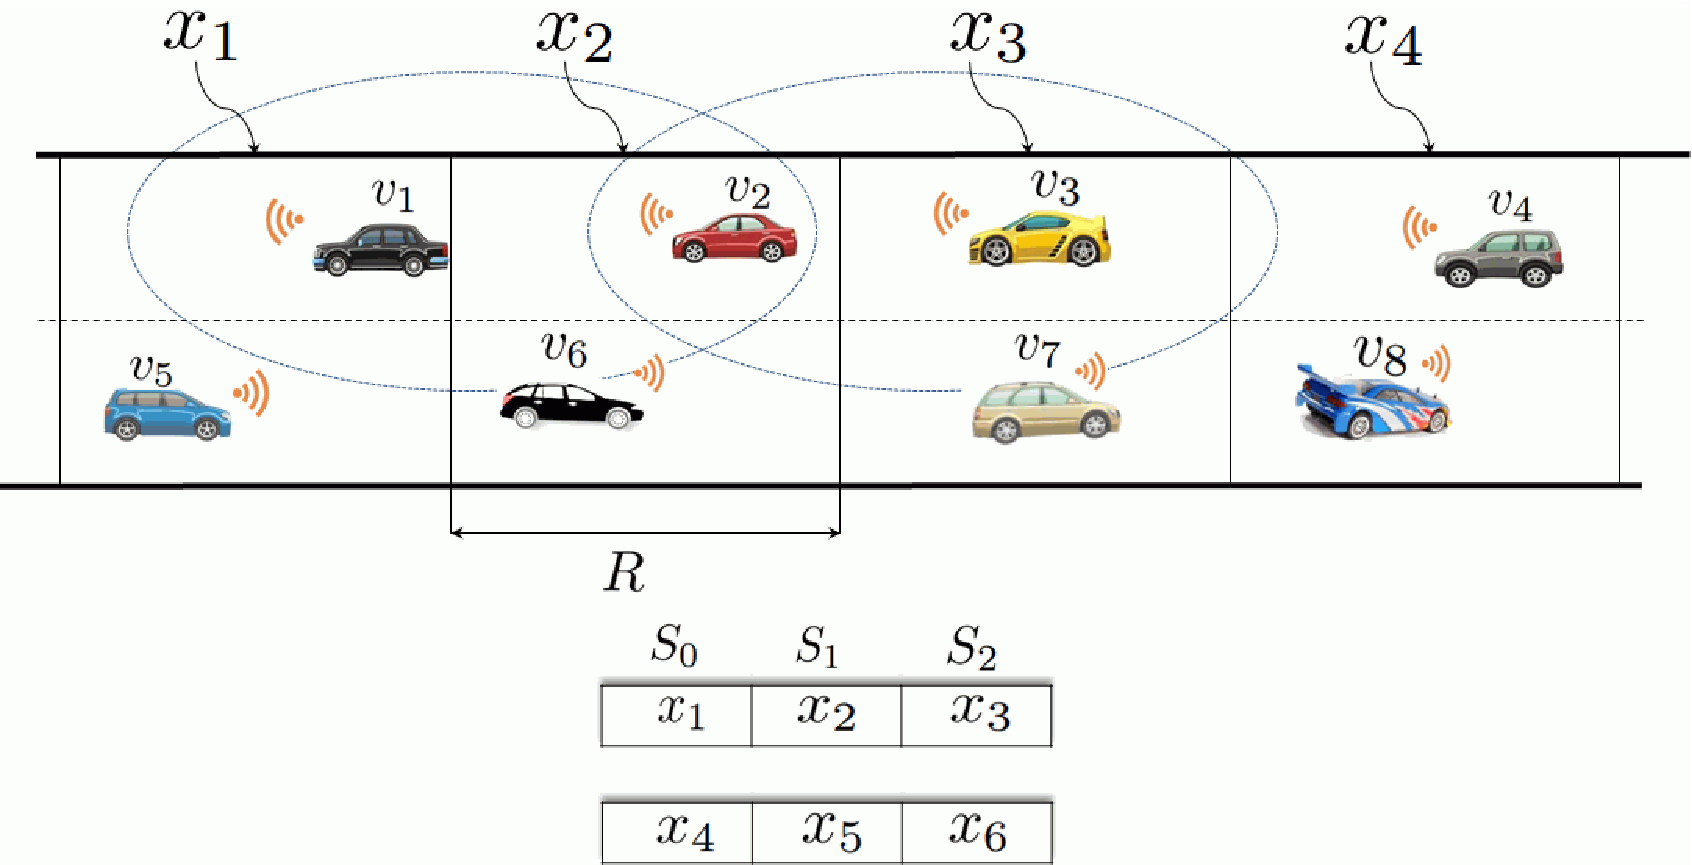
\includegraphics[height=7cm,width=14cm]{IMG/DTMAC_idea.pdf}
    \end{center}
    \caption{TDMA slots scheduling principle.}
    \label{figc:DTMAC_idea}
\end{figure}

The time slots in each TDMA frame are partitioned into three sets $S_0, S_1$ and $S_2$ associated with vehicles in three 
contiguous areas: $x_i, x_{i+1}$ and $x_{i+2}$, respectively (see Figure~\ref{figc:DTMAC_idea}). Each frame consists of a 
constant number of time slots, denoted by $\tau$ and each time slot is of a fixed time duration, denoted by $s$. Each vehicle 
can detect the start time of each frame as well as the start time of a time slot. In the VANET studied, all the vehicles are 
equipped with a GPS and thus the one-Pulse-Per-Second (1PPS) signal that a GPS receiver gets from GPS 
satellites can be used for slot synchronization. 

To prevent collisions on the transmission channel, our TDMA scheduling mechanism requires that every packet transmitted by 
any vehicle must contain additional information, called Frame Information (FI).
For the frame, this field gives the status of the slot (Idle, Busy, Collision) and 
the ID of the vehicles accessing each slot with the characteristic of the data 
sent: periodic or event-driven safety messages.

%The FI consists of a set of ID Fields (IDFs) of 
%size equal to the number of time slots per frame, $\tau$. Each IDF is dedicated to the corresponding time slot of a frame. The 
%basic FI structure is shown in Figure~\ref{figc:DTMAC_Frame}.
%Each time slot is dynamically reserved by an active vehicle 
%(the vehicle whose communication device is transmitting) for collision-free delivery of safety messages or other control messages.
%The VC\_ID field contains the ID of the vehicle that is accessing this slot. Each vehicle is identified by its MAC address. The 
%SLT\_STS field contains the status of each slot which indicates whether the slot is Idle, Busy or in Collision. Finally, the 
%PKT\_TYP field indicates the type of packet transmitted by the vehicle, i.e. periodic information or event-driven safety messages.
%
%\begin{figure}[!htbp]
%  \begin{center}
%  % Requires \usepackage{graphicx}
%  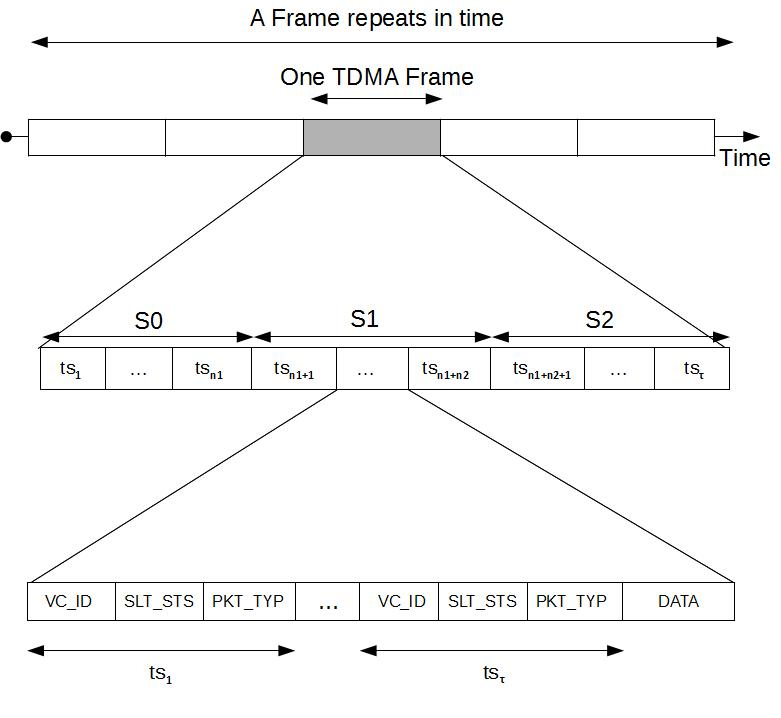
\includegraphics[height=10cm,width=13cm]{IMG/DTMACFrame.jpg}
%  \end{center}
%  \caption{Frame information (FI) structure.}
% \label{figc:DTMAC_Frame}
%\end{figure}
%
%Our distributed TDMA scheduling mechanism uses vehicles location and slot reuse concept to ensure that vehicles in 
%adjacent areas have collision-free schedule. The channel time is partitioned into frames and each frame is further 
%partitioned into three sets of time slots $S_0, S_1,$ and $S_2$ of size equal to $n1, n2~$and$~n3$, respectively. These sets 
%are associated with vehicles moving in the areas $x_i,~x_{i+1},~$and$~x_{i+2}$, respectively. As shown in 
%Figure~\ref{figc:DTMAC_idea}, by dividing the time slots into three sets, vehicles $v_1$ and $v_3$ that are moving 
%within the two areas $x_1$ and $x_3$, respectively, can not transmit simultaneously to  vehicle $v_2$ because they 
%are accessing disjoint sets of time slots. Therefore, our TDMA scheduling mechanism can decrease the collisions rate 
%caused by the hidden node problem. In each area, the vehicles access the time slots associated to their locations 
%with the same probability. In the rest of this chapter, we adopt the following notations:
%\begin{itemize}
%\item $S_{j}(v)$: The set of time slots associated to the area in which the vehicle $v$ is traveling. \vspace{1mm}
%\item $N(v)$: The set of neighbors\footnote{The set of neighbors is the set of vehicles that are moving within the same area.} of vehicle $v$ on the transmission channel. \vspace{1mm}
%\end{itemize}
%Every active vehicle in the network should be allocated a fixed slot in the frame for safety messages or other control 
%packet transmissions. It is obvious that a vehicle's slot cannot be used by any neighboring vehicles within the same area or in  adjacent areas, otherwise collisions will occur. The goal of this work is to propose an efficient slot reuse algorithm  without having to use expensive spectrum and complex broadband mechanisms such as FDMA or CDMA. In fact, the three subsets of time slots will be reused between neighboring areas in such a way no vehicle in different adjacent areas can access the channel at the same time, and thus no interference will occur. 
%
%
%Let us suppose that an active vehicle $v$ moving within the area $x_i$ needs to acquire a time slot on the transmission channel. Vehicle $v$ starts listening to the channel during the set of time slots reserved for the area in which it is traveling, let $S_{j}(v)$, where $j=(i+2)~mod~3$.
%
%\begin{itemize}
%
%\item Each vehicle that hears exactly one node transmission in a time slot reserved for its location, will set the status 
%of the slot to ''busy'' and record the ID of the vehicle accessing the channel in this time slot in the corresponding VC\_ID field.
%%\item Each vehicle that hears multiple FIs from different vehicles during the same time slot, will consider that the slot is occupied by more than one vehicle and sets its status to collision.
%\item If a vehicle does not hear anything during a specific time slot, it will set its status to ''free'' in the FI.
%\item If a vehicle can not decode the data during a specific time slot, it will set its status to ''collision'' in the FI.
%\item When a vehicle A has sent data in a given slot, it looks in the field information of the next slots to 
%discover whether its neighbors 
%have correctly received its data. If a neighbor of A reports  collision for this slot  (in the FI) or even if this slot is reported 
%to be ''busy'' 
%but being sent by another node (say B in the VC\_ID), A considers that its transmission has led to a 
%collision\footnote{Actually a node A considers that its transmission is a success if and only if all its neighbors 
%report a success in the FI of their slots specifying that the data was sent by node A.}. 
%\end{itemize}
%
%At the end of the frame the vehicle $v$ can determine the set $N(v)$ and the set of busy slots in $S_{j}(v)$ used by each 
%vehicle $u\in N(v)$, denoted by $B(v)$. In order to avoid any collision problem, this set of time slots can not be used by 
%any neighboring vehicles. Therefore,  vehicle $v$ can determine the set of available time slots $F(v)$ and then attempts to 
%select one of them at random, say time slot $k$.

The simulation results show that, compared to VeMAC which is the reference in terms of TDMA protocols for VANETs, DTMAC provides a lower rate of access and merging collisions, which results in significantly improved broadcast coverage. For further details see~\cite{hadded:hal-01379216}. 

% - - - - - - - - - - - - - -
\subsubsection{TRPM: a TDMA-aware routing protocol for multi-hop communications in VANETs}

\begin{participants}
    \pers{Mohamed}{Elhadad or Hadded}
    \pers{Paul}{Muhlethaler}
    \pers{Anis}{Laouiti}
\end{participants}

The main idea of TRPM is to select the next hop using the vehicle position and the time 
slot information from the TDMA scheduling.  Like the GPSR protocol, we assume that each transmitting vehicle 
knows the position of the packet's destination. In TRPM, the TDMA scheduling information and the position of a packet's destination 
are sufficient to make correct forwarding decisions at each transmitting vehicle. Specifically, if a  source vehicle is moving in 
area $x_i$, the locally optimal choice of next hop is the neighbor geographically located in area $x_{i+1}$ or $x_{i-1}$ according 
to the position of the packet's destination. As a result, the TDMA slot scheduling obtained by DTMAC  can be used to determine the 
set of next hops that are geographically closer to the destination. In fact, each vehicle that is moving in the area $x_i$ can 
know the locally optimal set of next hops that are located in adjacent areas $x_{i+1}$ or $x_{i-1}$ by observing the set of time 
slots $S_{(i+3)\%3}$ or $S_{(i+1)\%3}$, respectively. We consider the same example presented above when vehicle G as the destination 
vehicle that will broadcast a message received from vehicle A. As shown in Figure~\ref{figc:trpm}, only two relay vehicles are needed to ensure a 
multi-hop path between vehicle A and G (one relay node in the area $x_2$ and another one in the area $x_3$). 

\begin{figure}[H]
    \begin{center}
        % Requires \usepackage{graphicx}
        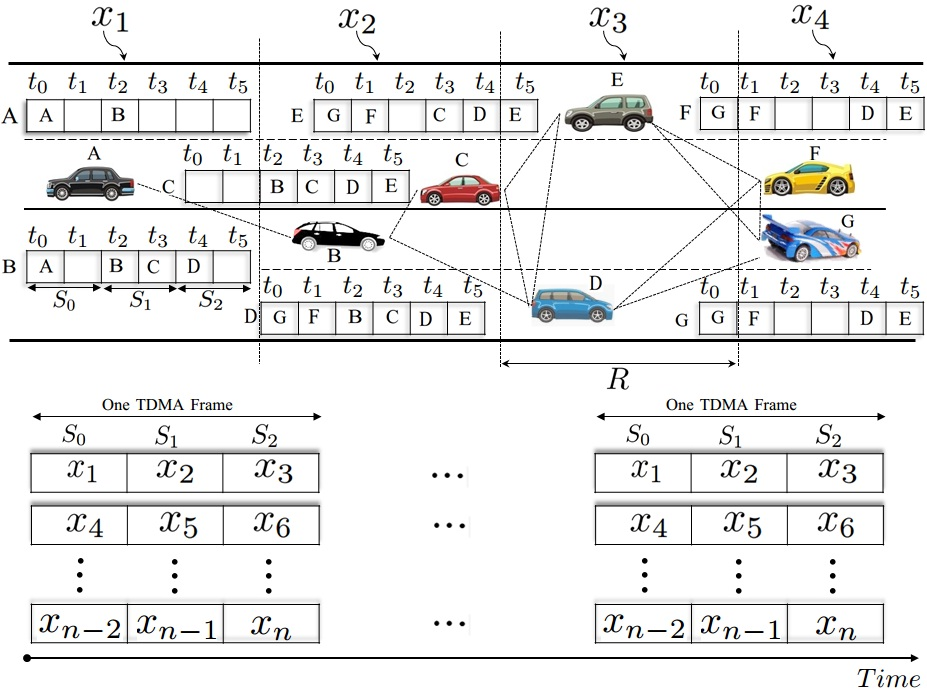
\includegraphics[height=9cm,width=15cm]{IMG/TRPM.jpg}
        \caption{VANET network using DTMAC scheduling scheme.}
        \label{figc:trpm}
    \end{center}
\end{figure}

In the following, the DTMAC protocol has been used by the vehicles to organize the channel access. The TDMA slot 
scheduling obtained by DTMAC is illustrated in Figure \ref{figc:trpm}. Firstly, vehicle A forwards a packet to B, as  vehicle A uses its frame 
information to choose a vehicle that is accessing the channel during the set $S_1$. Upon receiving the packet for forwarding, vehicle B 
will choose by using its frame information a vehicle that's accessing the channel during the set of time slots $S_2$ 
(say vehicle D). Then, vehicle D will forward the packet to G, as G is moving in area $x_4$ (accessing the channel during the 
set $S_0$) and it is the direct neighbor of vehicle D. By using DTMAC as the MAC layer, we can note that the path A-B-D-G is 
the shortest, in terms of the number of hops as well as the end-to-end delay which  is equal to 6 time slots  (2 time slots 
between $t_0$ and $t_2$ as $t_2$ is the transmission slot for vehicle B, then 2 time slots between $t_2$ and $t_4$ as $t_4$ is the 
transmission slot for vehicle D and finally 2 time slots between $t_4$ and $t_0$ as $t_0$ is the transmission slot in which vehicle 
G will broadcast the message received from  vehicle A). 

%%Packet forwarding algorithm

The idea of TRPM is the following. Whenever a vehicle $i$ accessing the channel during the set $S_k$ wants to send/forward an 
event-driven safety message, it constructs two sets of candidate forwarders based on its frame information FI as 
follows, where $TS(j)$ indicates the time slot reserved by vehicle $j$.

\begin{itemize}
    \item $A_i=\{j\in N(i)~|~TS(j)\in S_{(k+1)\%3}\}$ // \textit{The set of vehicles that are moving in the adjacent right-hand area.}
    \item $B_i=\{j\in N(i)~|~TS(j)\in S_{(k+2)\%3}\}$ // \textit{The set of vehicles that are moving in the adjacent left-hand area.}
\end{itemize}

Each source vehicle uses the position of a packet's destination and the TDMA scheduling information to make packet forwarding 
decisions. In fact, when a source vehicle $i$ is moving behind the destination vehicle, it will select a next hop relay that 
belongs to set $B_i$; when the transmitter is moving in front of the destination vehicle, it will select a forwarder vehicle 
from those in  set $A_i$. %Algorithm~\ref{ALGO1} outlines the behavior of our scheme during the procedure for sending an event-driven safety messages. 
For each vehicle $i$ that will send or forward a message, we define the normalized weight function WHS (Weighted next-Hop 
Selection) which depends on the delay and the distance between each neighboring vehicle $j$. WHS is calculated as follows:

\begin{center}
    \vspace{2mm}
    $WHS_{i,j}=\alpha*\frac{\Delta t_{i,j}}{\tau}-(1-\alpha)*\frac{d_{i,j}}{R}~~~~~~(1)$ 
    \vspace{2mm}
\end{center}

Where:

\begin{itemize}
    \item $\tau$ is the length of the TDMA frame (in number of time slots).
    \item $j$ is one of the neighbors of vehicle $i$, which represents the potential next hop that will relay the message received from vehicle $i$.
    \item $\Delta t_{i,j}$ is the gap between the sending slot of vehicle $i$ and the sending slot of vehicle $j$.
    \item $d_{i,j}$ is the distance between the two vehicles $i$ and $j$, and $R$ is the communication range. 
    \item $\alpha$ is a weighted value in the interval $[0,1]$ that gives more weight to either distance or delay. When $\alpha$ is high, more weight is given to the delay. Otherwise, when $\alpha$ is small, more weight is given to the distance.
\end{itemize}

We note that the two weight factors $\frac{\Delta t_{i,j}}{\tau}$ and $\frac{d_{i,j}}{R}$ are in conflict. For simplicity, we assume 
that all the factors should be minimized. In fact, the multiplication of the second weight factor
by (-1) allows us to transform a maximization to a minimization. Therefore, the forwarding vehicle for $i$ is the 
vehicle $j$ that is moving in an adjacent area for which $WHS_{i,j}$ is the lowest value.

The simulation results reveal that our routing protocol significantly outperforms other
protocols in terms of average end-to-end delay, average number
of relay vehicles and the average delivery ratio.

% - - - - - - - - - - - - - -
\subsubsection{CTMAC: a Centralized TDMA for VANETs}

\begin{participants}
    \pers{Mohamed}{Elhadad or Hadded}
    \pers{Paul}{Muhlethaler}
    \pers{Anis}{Laouiti}
\end{participants}
    
We have designed an infrastructure-based TDMA scheduling scheme which exploits the linear feature of VANET topologies. The 
vehicles' movements in a highway environment are linear due to the fact that their movements are constrained by the road topology. Our 
scheduling mechanism is also based on the assumption that the highway is equipped with some RSUs (i.e. one RSU 
for each $2\times R~meters$, where $R$ is the communication range). Note that each area is covered by one RSU installed on 
the side of the highway and in the middle of the corresponding area. The time slots in each TDMA 
frame are partitioned into two sets $S_1, S_2$ associated with vehicles in two adjacent RSU 
areas (see Figure~\ref{fig:CTSA}). Each frame consists of a constant number of time slots, denoted by $\tau$ and each time 
slot is of a fixed time duration, denoted by $s$. Each vehicle can detect the start time of each frame as well as the 
start time of a time slot. 
%In the VANET studied, all the vehicles are equipped with a GPS 
%and thus the one-Pulse-Per-Second (1PPS) signal that a GPS receiver gets from GPS satellites can be used for 
%slot synchronization. The first time slot either in the set $S_1$ or $S_2$ is always used by the correspondent RSU to
%broadcast a Slot Announcement message (SA) to the vehicles within its coverage area. In the following, we detail the slot scheduling mechanism in CTMAC and we show how this protocol can 
%provide an efficient time slot utilization for the participating vehicles, while minimizing transmission collisions caused 
%by the hidden node problem.

\begin{figure}[!htbp]
    \begin{center}
        % Requires \usepackage{graphicx}
        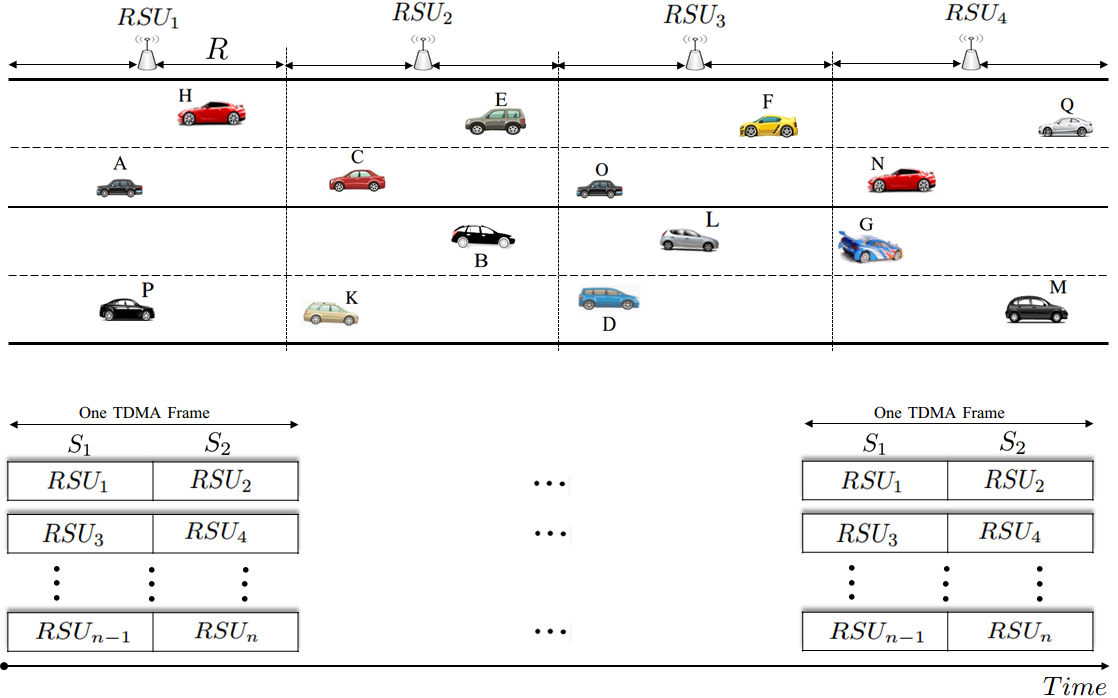
\includegraphics[height=8cm,width=14cm]{IMG/CTMACprinciple.png}
        \caption{TDMA slots scheduling mechanism of CTMAC}
        \label{fig:CTSA}
    \end{center}
\end{figure}

The CTMAC scheduling mechanism uses a slot reuse concept 
to ensure that vehicles in adjacent areas covered by two RSUs have 
a collision-free schedule. The channel time is partitioned into frames and
each frame is further partitioned into two sets of time slots $S_1$ and $S_2$. 
These sets are associated with vehicles moving in the adjacent RSU areas. 
These sets of time slots are reused along the highway in such a way that no vehicles belonging to 
the same set of two-hop 
neighbors using the same time slot. As shown in Figure~\ref{fig:CTSA}, the vehicles in 
the coverage area of $RSU_1$ and those in the coverage area of $RSU_2$ are
accessing disjoint sets of time slots. As a result, the scheduling mechanism of 
CTMAC can decrease the collision rate by avoiding the inter-RSUs interference 
without using any complex band.  Each active vehicle keeps accessing the same 
time slot on all subsequent frames unless it enters another area covered by another 
RSU or a merging collision problem occurs. Each vehicle uses only its allocated 
time slot to transmit its packet on the control channel.

The simulation results
reveal that CTMAC significantly outperforms the VeMAC and
ADHOC MAC protocols. in terms of transmission collisions
and the overhead required to create and maintain the TDMA
schedules, see~\cite{hadded:hal-01379219}. 

%  \begin{figure}[!h]
%  \begin{center}
%  % Requires \usepackage{graphicx}
% 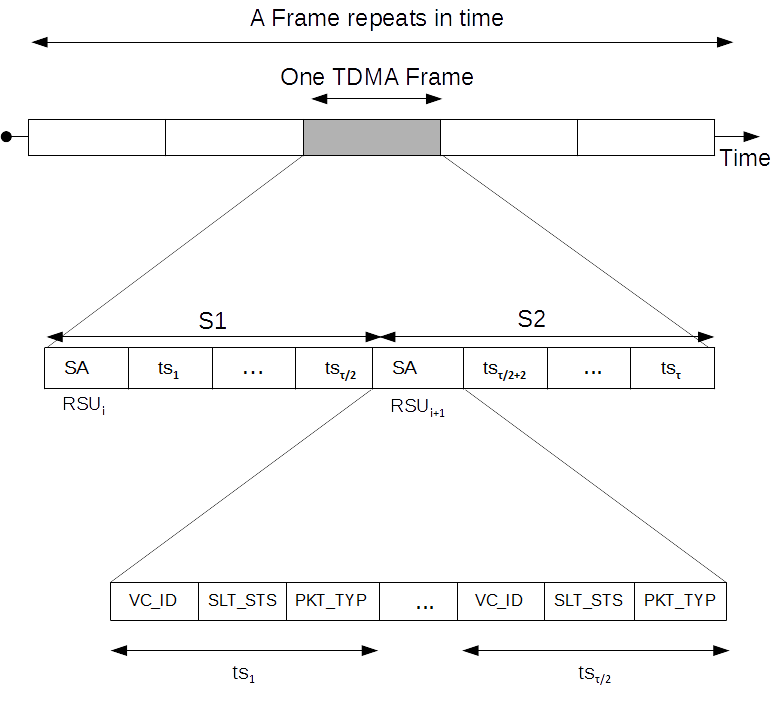
\includegraphics[height=10cm,width=15cm]{IMG/CTMACFrame.jpg}
%  \caption{Frame information (FI) structure.}
% \label{fig:CTSA_FI}
%  \end{center}
%\end{figure}
%
%In CTMAC, each RSU constructs and maintains a Frame Information (FI) 
%of length equal to the number of time slots per frame, $\tau$. 
%For the frame, this field gives the status of the slot (Idle, Busy, Collision) and 
%the ID of the vehicles accessing each slot with the characteristic of the data 
%sent: periodic or event-driven safety messages. 
%
%The FI consists 
%of a set of ID Fields (IDFs) and each one is dedicated to the corresponding 
%time slot of a frame. The FI structure is shown in Figure~\ref{fig:CTSA_FI}. 
%Each IDF consists of three fields: VC\_ID, SLT\_STS and PKT\_TYP. 
%The VC\_ID field contains the ID of the vehicle that is accessing this slot. 
%The SLT\_STS field contains the status of each slot which indicates whether 
%the slot is Idle, Busy or in Collision. Finally, the PKT\_TYP field indicates 
%the type of packet transmitted by the vehicle, i.e. periodic information or 
%event-driven safety messages. Unlike the VeMAC and ADHOC MAC 
%protocols, in the CTMAC protocol, only the RSU nodes periodically 
%broadcast their frame information and each vehicle will update its frame
% information based on the packet transmitted by its RSU. However, a 
% vehicle broadcasts its frame information only when an access collision problem is detected. 
%
%At the end of each frame, each RSU $u$ can determine the set of 
%free time slots based on its frame information, denoted by $F(u)$. 
%When an RSU has one or more available time slots, it announces that 
%by broadcasting a Slot Announcement (SA) message containing its 
%identity $(SA->NODE\_ID)$ to all the vehicles in its coverage area. 

%\begin{algorithm}[!htbp]
%\caption{Action at each vehicle that will reserve a time slot}\label{SlotReservation}
%\textbf{Input~~} \\
%$S_{j}(v):$ the set of time slots that the vehicle $v$ can reserve.\\
%$\alpha_j,~\beta_j$: are the indexes of the first and the last slot of the set $S_{j}(v)$, respectively. 

%\begin{algorithmic}[1]
%
%\STATE ~//~TDMA slot assignment
%\IF{\textit{vehicle $v$ receives an SA message from RSU $u$}}
%\STATE \textit{$MY\_RSU\_ID=SA->NODE\_ID$}
%\STATE \textit{vehicle $v$ randomly reserves a temporary time slot, say slot $k$.}
%\STATE \textit{vehicle $v$ sends a SREQ to RSU $u$ during the time slot $k$.}
%\ENDIF
%\WHILE{$timer_1!=0$}
%\IF{\textit{vehicle $v$ receives an SREP message from RSU $u$}}
%\STATE \textit{vehicle $v$ starts to broadcast its message during the time slot \textit{$SREP->SLT\_ID.$}}
%\ENDIF  
%\ENDWHILE
%\IF{$(time_1==0)~and~(TS(v)==\emptyset)$}
%\STATE \textit{go to 2.}
%\ENDIF
%\STATE ~//~TDMA schedule maintenance
%\WHILE{$TS(v)!=\emptyset$}
%\IF{\textit{$MY\_RSU\_ID!=SA->NODE\_ID$}}
%\STATE \textit{go to 2.}
%\ENDIF   
%\ENDWHILE
%\end{algorithmic}
%\end{algorithm}

%When a vehicle receives 
%an SA message, and if it wishes to access the channel, it tries to get the 
%%attention of the RSU by sending it a Slot REQuest message (SREQ) including its identity. Algorithm~\ref{SlotReservation} outlines the details of the slot 
%%reservation mechanism.
% $v$ represents the vehicle that needs to reserve a 
%time slot, $timer_1$ is a timer and $TS(v)$ is the time slot that is successfully 
%acquired by vehicle $v$. When an RSU receives the SERQ message, it checks 
%whether there is an available time slot and, if there is, the RSU sends a Slot REPly 
%message (SREP) to the corresponding vehicle including the slot index $(SREP->SLT\_ID)$. 
%After the reception of the SREP, the vehicle $v$ starts to broadcast its message 
%during its time slot, $TS(v)=SREP->SLT\_ID$. Otherwise, if the timer expires and 
%no response has been received from the RSU (lines 12-14), the vehicle $v$ will repeat the same steps.
%If a vehicle receives an SA message from another RSU (line 17), the vehicle 
%will send an SREQ to allocate a new time slot and if it receives an SREP from 
%the RSU it will release its current time slot and it will start to broadcast its packet 
%during the time slot allocated by the new RSU. Moreover, when an RSU does 
%not receive a message from a vehicle $v$ during its slot, it considers that it has 
%left its coverage area and it releases its time slot. 

%Algorithm~\ref{SlotScheduling} 
%outlines the behavior of our scheme during the procedure of slot scheduling at the RSU.  

%\begin{algorithm}[!htbp]
%\caption{Slot scheduling procedure executed at each RSU}\label{SlotScheduling}
%$\alpha_j,~\beta_j$: are the indexes of the first and the last slot of the set $S_{j}(v)$, respectively. 
%\begin{algorithmic}[1]
%\STATE \textbf{Input:} 
%\STATE \textit{$S_{j}:$ The set of time slots managed by the RSU $u$.}
%\IF{\textit{current\_slot$==TS(u)$ and $F(u)\neq\{\emptyset\}$}}
%\STATE \textit{$u$ broadcasts an SA message.}
%\ENDIF
%
%\IF{\textit{$u$ receives an SREQ message from vehicle $v$}}
%\IF{\textit{$\exists~k \in S_j$ such that FI[k].SLT\_STS=Free}}    
%\STATE \textit{$u$ allocates the slot $k$ to vehicle $v$.}
%\STATE \textit{$u$ sends a SREP to vehicle $v$.}
%\ENDIF
%\ENDIF
%\WHILE{true}
%\IF{\textit{$u$ detects that there is a vehicle has leaved its coverage area, say vehicle $i$}}
%\STATE \textit{ FI[TS($i$)].SLT\_STS=Free}
%\ENDIF   
%\ENDWHILE

%\end{algorithmic}
%\end{algorithm}

% - - - - - - - - - - - - - -
\subsubsection{A Flooding-Based Location Service in VANETs}

\begin{participants}
    \pers{Selma}{Boumerdassi}
    \pers{Paul}{Muhlethaler}
    \pers{Eric}{Renault}
\end{participants}

We have designed and analyzed a location service for VANETs; 
such a service can be used in Location-based routing protocols for 
VANETs. Our protocol is  a proactive
flooding-based location service that drastically reduces the
number of update packets sent over the network as compared to
traditional flooding-based location services. This goal is achieved
by partially forwarding location information at each node. A
mathematical model and some simulations are proposed to show
the effectiveness of this solution. Cases for 1D, 2D and 3D spaces
are studied for both deterministic and probabilistic forwarding
decisions. We compare our protocol with the Multi-Point Relay (MPR) 
technique which is used in the OLSR protocol and determine the best  technique 
according to the network conditions.  

%------------------------------------------------------------------------------
\subsection{Models for Wireless Networks and VANETs}

%\begin{participants}
%    \pers{Nadjib}{Achir}
%    \pers{Younes}{Bouchaala}
%    \pers{Guy}{Fayolle}
%    \pers{Paul}{Muhlethaler}
%    \pers{Oyunchimeg}{Shagdar}
%\end{participants}

% - - - - - - - - - - - - - -
\subsubsection{Performance analysis of IEEE 802.11 broadcast schemes with different inter-frame spacings}

\begin{participants}
    \pers{Younes}{Bouchaala}
    \pers{Paul}{Muhlethaler}
    \pers{Oyunchimeg}{Shagdar}
    \pers{Nadjib}{Achir}
\end{participants}

We have started to build a model which analyzes the performance 
of IEEE 802.11p managing different classes of priorities. 
The differentiation of traffic streams is obtained with different 
inter-frame spacings:  AIFSs (for Arbitration Inter Frame Spacings) and with 
different back-off windows: CWs (for Collision Windows). 
This model is based on a Markov model where the state is the remaining 
number of idle slots that a packet of a given class has to wait before transmission. 
However, in addition to this Markov model for which we compute a steady state 
we also consider the Markov chain which counts the number of idle slots after 
the smallest AIFS. As a matter of fact the probability these states are not evenly 
distributed since with different AIFSs the arrival rate is not constant 
when the number of idle slots experienced after the smallest AIFS varies. 
The resolution of the steady state of these two inter-mixed Markov chains
lead to non linear and intertwined equations that can be easily  solved with a software 
such as Maple. 
With the model we have obtained, we can compute the delivery rate 
of packets of different classes and show the influence of system parameters: 
AIFSs and CWs. The preliminary results show a a very strong influence 
of different AIFSs on the performance for each traffic streams.  

% - - - - - - - - - - - - - -
\subsubsection{Model of IEEE 802.11 Broadcast Scheme with Infinite Queue}

\begin{participants}
    \pers{Guy}{Fayolle}
    \pers{Paul}{Muhlethaler}
\end{participants}

We have analyzed the so-called back-off technique of the IEEE 802.11 protocol
in broadcast mode with waiting queues. In contrast to existing models, packets arriving when a
station (or node) is in back-off state are not discarded, but are stored in a buffer of infinite capacity.
As in previous studies, the key point of our analysis hinges on the assumption that the time on
the channel is viewed as a random succession of transmission slots (whose duration corresponds
to the length of a packet) and mini-slots during which the back-off of the station is decremented.
These events occur independently, with given probabilities. The state of a node is represented by a
two-dimensional Markov chain in discrete-time, formed by the back-off counter and the number of
packets at the station. Two models are proposed both of which are shown to cope reasonably well
with the physical principles of the protocol. The stability (ergodicity) conditions are obtained and
interpreted in terms of maximum throughput. Several approximations related to these models are
also discussed. The results of this study are in \cite{fayolle:hal-01166082}. 

% - - - - - - - - - - - - - -
\subsubsection{Model and optimization of CSMA}

\begin{participants}
    \pers{Younes}{Bouchaala}
    \pers{Paul}{Muhlethaler}
    \pers{Oyunchimeg}{Shagdar}
    \pers{Nadjib}{Achir}
\end{participants}

We have studied  the maximum throughput of CSMA in scenarios with spatial reuse.
The nodes of our network form a Poisson Point Process (PPP) of a one- or two-dimensional space.
The one-dimensional PPP well represents VANETs.
To model the effect of Carrier Sense Multiple Access (CSMA), we give random marks to our nodes and to elect transmitting nodes in the PPP we choose the nodes with the smallest marks in their neighborhood, this is the Matern hardcore selection process.
To describe the signal propagation, we use a signal with power-law decay and we add a random Rayleigh fading.
To decide whether or not a transmission is successful, we adopt the Signal-over-Interference Ratio (SIR) model in which a packet is correctly received if its transmission power divided by the interference power is above a capture threshold.
We assume that each node in our PPP has a random receiver at a typical distance.
We choose the average distance to its closest neighbor.
We also assume that all the network nodes always have a pending packet.
With these assumptions, we analytically study the density of throughput of successful transmissions and we show that it can be optimized with the carrier-sense threshold. 
 The model makes it possible to analytically compute the 
 performance of a CSMA system and gives 
 interesting results on the network performance such as the capture probability 
 when the throughput is optimized, and the effect on a non-optimization of the 
 carrier sense threshold on the throughput. We can also study the influence 
of the parameters and  see their effects on the overall performance. 
We observe a significant difference between 2D an 1D networks.

We have built two models  to compare the spatial density of successful 
transmissions of CSMA and Aloha. 
To carry out a  fair comparison, we optimize both schemes by adjusting their parameters. 
For spatial Aloha, we can adapt the 
transmission probability, whereas for spatial CSMA we have to find the suitable carrier sense threshold. The results obtained show that CSMA, when optimized, outperforms Aloha 
for nearly all the parameters of the network model values 
and we evaluate the gain of CSMA over Aloha. 
We also find interesting results concerning the effect of the model parameters on the performance 
of both Aloha and CSMA. 
The closed formulas we have obtained provide immediate evaluation of performance, whereas 
simulations may take minutes to give their results. Even if Aloha and CSMA are not recent protocols, 
this comparison of spatial performance is new and provides interesting and useful results. 

For Aloha networks, when we study transmissions over the average distance to the closest 
neighbor, the optimization does not depend on the density of nodes, 
which is a very interesting property. Thus in Aloha networks, the density of 
successful transmissions easily scales linearly in $\lambda$ when we vary 
$\lambda$ whereas in CSMA networks the protocol must be carefully 
tuned to obtain this scaling. 

% - - - - - - - - - - - - - -
\subsubsection{Adaptive CSMA}

\begin{participants}
     \pers{Nadjib}{Achir}
    \pers{Younes}{Bouchaala}
    \pers{Paul}{Muhlethaler}
    \pers{Oyunchimeg}{Shagdar}
\end{participants}

Using the model we have built for CSMA, we have shown that when optimized 
with the carrier sense detection threshold $P_{cs}$, 
the probability $p^*$ of transmission for a node 
in the CSMA network does not depend on the density of nodes $\lambda$. 
In other words when the CSMA is optimized to obtain the largest density of successful 
transmissions (communication from nodes to their neighbors), $p^*$  is constant.
We have verified this statement 
on several examples and we think that a formal proof of this remark is possible using 
scaling  arguments. The average access delay is a direct function of the probability of transmission $p$. Thus the average delay when the carrier sense detection threshold is optimized 
is a constant $D_{target}$ which does not depend on $\lambda$. 
A stabilization algorithm which 
adapts $P_{cs}$ to reach the $D_{target}$ can thus be envisioned. 

\end{module} 

%==============================================================================
%\begin{module}{resultats}{results:modelswireless}{Models for wireless networks}

%------------------------------------------------------------------------------
%\subsection{Interference and SINR coverage in spatial non-slotted Aloha networks}
%
%\begin{participants}
%    \pers{Bartek}{Blaszczyszyn}
%    \pers{Paul}{Muhlethaler}
%\end{participants}
%
%
%We propose two analytically tractable stochastic-geometric models of interference in adhoc
%networks using pure (non-slotted) Aloha as the medium access. In contrast the slotted model, the interference in
%pure Aloha may vary during the transmission of a tagged
%packet. We develop closed form expressions for the Laplace
%transform of the empirical average of the interference
%experienced during the transmission of a typical packet.
%Both models assume a power-law path-loss function with
%arbitrarily distributed fading and feature configurations
%of transmitters randomly located in the Euclidean plane
%according to a Poisson point process. Depending on the
%model, these configurations vary over time or are static. We
%apply our analysis of the interference to study the Signal-to-
%Interference-and-Noise Ratio (SINR) outage probability for
%a typical transmission in pure Aloha. The results are used
%to compare the performance of non-slotted Aloha to the
%slotted one, which has almost exclusively been previously
%studied in context of wired ad-hoc networks.
%
%------------------------------------------------------------------------------
%\subsection{Random linear multihop relaying in a general field of interferers using spatial Aloha }
%
%\begin{participants}
%    \pers{Bartek}{Blaszczyszyn}
%    \pers{Paul}{Muhlethaler}
%\end{participants}
%
%We study a stationary Poisson
%pattern of nodes on a line embedded in an independent planar
%Poisson field of interfering nodes. Assuming slotted Aloha and
%the signal-to-interference-and-noise ratio capture condition, with
%the usual power-law path loss model and Rayleigh fading, we
%explicitly evaluate several local and end-to-end performance
%characteristics related to the nearest-neighbor packet relaying on
%this line, and study their dependence on the model parameters
%(the density of relaying and interfering nodes, Aloha tuning and
%the external noise power). Our model can be applied in two cases:
%the first use is for vehicular ad-hoc networks, where vehicles are
%randomly located on a straight road. The second use is to study
%a “typical” route traced in a (general) planar ad-hoc network by
%some routing mechanism. The approach we have chosen allows
%us to quantify the non-efficiency of long-distance routing in “pure
%ad-hoc” networks and evaluate a possible remedy for it in the
%form of additional “fixed” relaying nodes, called road-side units in
%a vehicular network. It also allows us to consider a more general
%field of interfering nodes and study the impact of the clustering
%of its nodes on the routing performance. As a special case of
%a field with more clustering than the Poison field, we consider
%a Poisson-line field of interfering nodes, in which all the nodes
%are randomly located on random straight lines. In this case our
%analysis rigorously (in the sense of Palm theory) corresponds to
%the typical route of this network. The comparison to our basic
%model reveals a paradox: clustering of interfering nodes decreases
%the outage probability of a single (typical) transmission on the
%route, but increases the mean end-to-end delay
%
%\end{module}

%==============================================================================
%%\begin{module}{resultats}{new2}{New result 2}
%%ICI Vous pouvez ecrire du texte
%%\end{module}

%%%%%%%%%%%%%%%%%%%%%%%%%%%%%%%%%%%%%%%%%%%%%%%%%%%%%%%
%%%
%%% Section contrats (Bilateral Contracts and Grants with Industry)
%%% Il y a des modules ici
%%%
%%%%%%%%%%%%%%%%%%%%%%%%%%%%%%%%%%%%%%%%%%%%%%%%%%%%%%%

%%% https://intranet.inria.fr/Vie-scientifique/Information-edition-scientifiques/Comment-rediger-le-RAweb/Les-sections#eztoc27554_11

%==============================================================================
\begin{module}{contrats}{cgwi1}{Bilateral Contracts with Industry}

%------------------------------------------------------------------------------
\subsection{CNES}

\begin{participants}
    \pers{Ines}{Khoufi}
    \pers{Pascale}{Minet}
    \pers{Erwan}{Livolant}
\end{participants}

Partners: CNES, Inria.\\

Following the SAHARA project that ended in 2015, CNES decided to fund a study about the use of wireless sensor networks in space environment.
This new project started in November 2015 and will end in November 2016.

For CNES we studied how to use a IEEE 802.15.4e TSCH (Time Slotted Channel Hopping) network in the space launch vehicles. We proposed new solutions and evaluated their performances with the NS3 simulation tool.\\

\end{module}

%==============================================================================
\begin{module}{contrats}{cgwi2}{Bilateral Grants with Industry}

%------------------------------------------------------------------------------
\subsection{Gridbee CIFRE}

\begin{participants}
    \pers{Thomas}{Watteyne}
    \pers{Jonathan}{Mu\~noz}
\end{participants}

\begin{itemize}
    \item Title: km-scale Industrial Networking
    \item Type: CIFRE agreement
    \item Period: Nov 2015 - Oct 2018
    \item Coordinator: \thomas
    \item Goal: CIFRE agreement with Gridbee (\url{http://www.gridbeecom.com/}) to apply 6TiSCH-style scheduling on top of long-range IEEE802.15.4g radios. Implementation of those solutions on OpenWSN.
\end{itemize}

\end{module}

%%%%%%%%%%%%%%%%%%%%%%%%%%%%%%%%%%%%%%%%%%%%%%%%%%%%%%%%%%%%%%%%%
%%%
%%% Section partenariat (Partnerships and Cooperations)
%%% Il y a des modules ici
%%%
%%% Dans cette section, certains modules sont **normalises**.
%%% Par consequent, la liste de ces modules
%%% est :
%%% 
%%% \begin{module}{partenariat}{regional}{Regional Initiatives}
%%% \begin{module}{partenariat}{national}{National Initiatives}
%%% \begin{module}{partenariat}{europe}{European Initiatives}
%%% \begin{module}{partenariat}{international}{International Initiatives}
%%% \begin{module}{partenariat}{visites}{International Research Visitors}
%%% 
%%% On peut, en outre, ajouter des modules pour inserer ce qui ne 
%%% rentre pas dans les categories ci-dessus. Pour chacun des modules 
%%% listes, les actions proprement dites apparaitront en 
%%% \subsubsection, et les listes de {participants} seront ventilees en 
%%% consequence, par \subsubsection (et non plus par module)
%%% 
%%%%%%%%%%%%%%%%%%%%%%%%%%%%%%%%%%%%%%%%%%%%%%%%%%%%%%%%%%%%%%%%%%%

%%% https://intranet.inria.fr/Vie-scientifique/Information-edition-scientifiques/Comment-rediger-le-RAweb/Les-sections#eztoc27554_12
%\begin{module}{partenariat}{regional}{Regional Initiatives}
%% ICI Vous pouvez ecrire du text
%\end{module}

%==============================================================================
\begin{module}{partenariat}{national}{National Initiatives}

%%% Présentez vos données avec les items en précisant pour chaque projet : 
%%% Project Acronym, Project Title, Coordinator, Duration, Others Partners, Abstract... 

%------------------------------------------------------------------------------
%\subsection{ANR}

%EVA has currently no ANR project but plan to submit an ASTRID project in 2016. 

%------------------------------------------------------------------------------ 
\subsection{Competitivity Clusters}

% - - - - - - - - - - - - - -
\subsubsection{SAHARA}

\begin{participants}
    \pers{Pascale}{Minet}
    %\pers{Ridha}{Soua}
    \pers{Erwan}{Livolant}
\end{participants}

Period: 2011 - 2016.

Partners: EADS (coordinator), Astrium, BeanAir, CNES, ECE, EPMI, Eurocopter, GlobalSys, Inria, LIMOS, Oktal SE, Reflex CES, Safran Engineering Systems.

SAHARA is a FUI project, labelled by ASTECH and PEGASE, which aims at designing a wireless sensor network embedded in an aircraft. The proposed solution should improve the embedded mass, the end-to-end delays, the cost and performance in the transfers of non critical data. 

This project ended in March 2016. After a presentation of the SAHARA project at the IEEE WISEE 2015 conference (Wireless for Space and Extreme Environments), we were selected to write a book chapter entitled "Multichannel Wireless Sensor Networks for Aircraft: Challenges and Issues" in the Wiley book
"Wireless sensor systems for extreme environments: space, underwater, underground and industrial". 

% - - - - - - - - - - - - - -
\subsubsection{CONNEXION}

\begin{participants}
    \pers{Pascale}{Minet}
    \pers{Ines}{Khoufi}
    \pers{Erwan}{Livolant}
\end{participants}

Period: 2012 - 2016.

Partners: EDF (coordinator), All4Tec, ALSTOM, AREVA, Atos WorldGrid, CEA, CNRS / CRAN, Corys TESS, ENS Cachan, Esterel Technologies, Inria, LIG, Predict, Rolls-Royce Civil Nuclear, Telecom ParisTech.

The Cluster CONNEXION (Digital Command Control for Nuclear EXport and renovatION) project aims to propose and validate an innovative architecture platforms suitable control systems for nuclear power plants in France and abroad. This architecture integrates a set of technological components developed by the academic partners (CEA, Inria, CNRS / CRAN, ENS Cachan, LIG, Telecom ParisTech) and based on collaborations between major integrators such as ALSTOM and AREVA, the operator EDF in France and ``techno-providers'' of embedded software (Atos WorldGrid, Rolls-Royce Civil Nuclear, Corys TESS, Esterel Technologies, All4Tec, Predict).
With the support of the competitiveness clusters System@tic, Minalogic and Burgundy Nuclear Partnership,the project started in April 2012. The key deliverables of the project covered several topics related demonstration concern-driven engineering models for the design and validation of large technical systems, design environments and evaluation of HMI, the implementation of Wireless Sensor Network context-nuclear, buses business object or real-time middleware facilitating the exchange of heterogeneous data and distributed data models standardized to ensure consistency of digital systems. 

The EVA team focuses more particularly on the interconnection of the OCARI wireless sensor network with the industrial facility backbone and deployment algorithms of wireless sensors.


In the Cluster Connexion project, the goal for the EVA team was to design and implement new functionnalities for the OCARI wireless sensor network to allow it to:

\begin{itemize}
    \item support the mobility of some sensor nodes (targeted application: remote dosimetry to monitor the exposition of people to radiations), 
    \item transmit commands to sensors/actuators (e.g. configuration parameters, regeneration order),
    \item ensure data gathering during node recoloring,  
    \item remotely manage the parameters of the OCARI network,
    \item aggregate in a single frame several heterogeneous measures originated from different sensors on a same wireless node, 
    \item use a generic format for the measures: type, length, value.
    \item integrate this network to the middleware of context-aware services, OPC-UA/ROSA. 
\end{itemize}

The demonstrator "a mobile connected worksite" developed in the Cluster Connexion project meets several objectives:
\begin{itemize}
    \item Make the wireless sensor networks more reliable in an  ionisating environment ionisant;
    \item Make easier the diagnostic and the repairing by means of the aggregation of data originated from heterogeneous sources; 
    \item Take into account the requirements of information security in the architectures;
    \item Ensure a continuum of solutions for the industrial involved.\\
\end{itemize}

The Industrial IoT (Internet of Things) solution proposed by Connexion is an integrated chain, from the wireless sensor\& actuator network up to the surveillance, diagnostic and health infrastructure monitoring applications, using a context-aware middleware fitting the industrial environment.\\ 

At the end of the Cluster Connexion project, we made the demonstration of a command/control loop for the regeneration of wireless sensor nodes in collaboration with CEA, Predict, Telecom ParisTech, EDF, ATOS and Inria highlighting the following steps:

\begin{itemize}
    \item the upstream flow of health indicators from electronic devices,
    \item detection of an abnormal behavior by a monitoring software (KASEM),  
    \item generation of a regeneration command and transmission of this command to the misbehaving sensor node.
    \item regeneration of the involved sensor
    \item insertion of the regenerated sensor in the OCARI network.\\
\end{itemize}

When the Cluster Connexion project ended, the results obtained with regard to the OCARI network and the OPC-UA/ROSA middleware have been transferred to the Task Force ConnexSensors hosted by AFNeT. The goals of the ConnexSensors TaskForce are:

\begin{itemize}
    \item Federate industrial companies around an IoT solution IoT including wireless sensor \& actuator networks and a standardized industrial middleware.
    \item Jointly valorize the OCARI wireless sensor \& actuator network and the OPC-UA/ROSA middleware.
    \item Deploy the Connexion demonstrator in the basemenet of interested industrials. 
    \item Ensure that industrials will keep the mastership of their data. 
    \item Ensure the perennity of the solution proposed.\\
\end{itemize}

%------------------------------------------------------------------------------
\subsection{Other collaborations}

EVA has a collaboration with Vedecom. 
\paul~supervises Younes Bouchaala's PhD funded by Vedecom. This PhD aims at 
studying vehicle-to-vehicle communication to improve roads safety. 

\end{module} 

%%%%%%%%%%%%%%%%%%%%%%%%%%%%%%%%%%%%%%%%%%%%%%%%%%%%%%%%%%%%%%%%%%%%%%
%%%
%%% Information sur les données importées : projets européens
%%%  
%%% Les données sur vos partenariats européens sont issus de la DPEI via l'entrepôt de données. 
%%% Les données affichées sont : Nom du projet, Type Defi, 
%%%                              Instrument, Duration, Coordinator, Others partners.
%%%
%%% Complétez ce qui manque : résumé, Others partners (on attend des noms de pays), ... 
%%%
%%% En cas de problème : raweb-support@inria.fr 
%%%
%%%%%%%%%%%%%%%%%%%%%%%%%%%%%%%%%%%%%%%%%%%%%%%%%%%%%%%%%%%%%%%%%%%%%%

%==============================================================================
\begin{module}{partenariat}{europe}{European Initiatives}

%%% En savoir plus : https://intranet.inria.fr/Vie-scientifique/Information-edition-scientifiques/Comment-rediger-le-RAweb/Les-sections#eztoc27554_14

%------------------------------------------------------------------------------
\subsection{H2020 Projects}

% - - - - - - - - - - - - - -
\subsubsection{F-Interop}

\begin{itemize}
    \XMLaddatt*{type}{sanspuces}
    \item Type: H2020
    \item Objective: Design and implement a cloud-based interoperability testing platform for low-power wireless standards.
    \item Duration: Nov 2015 - Oct 2017
    \item Coordinator: UPMC (FR)
    \item Other partners: iMinds (BE), ETSI (FR), EANTC (DE), Mandat International (CH), DigiCat (UK), UL (LU), Inria (FR), Device Gateway (CH)
    \item Inria contact: \thomas
\end{itemize}

% - - - - - - - - - - - - - -
\subsubsection{ARMOUR}

\begin{itemize}
    \XMLaddatt*{type}{sanspuces}
    \item Type: H2020
    \item Objective: Security for the IoT
    \item Duration: Dec 2015 – Nov 2017
    \item Coordinator: UPMC (FR)
    \item Other partners: Inria (FR), Synelixis (EL), Smartesting (FR), Unparallel (PT), JRC (BE), Ease Global Market (FR), Odin Solutions (ES)
    \item Inria-EVA contact: \thomas
\end{itemize}

% - - - - - - - - - - - - - -
\subsubsection{Project Reviewing} 

\begin{itemize}
    \item \paul~was reviewer for the E3Network project  (E-band transceiver for the backhaul infrastructure of the future networks). The transceiver designed in the E3Network project will use modern digital multi-level modulations to achieve high spectral efficiency. This together with the huge bandwidth will enable high capacities above 10 Gbps.
\end{itemize}

%------------------------------------------------------------------------------
\subsection{Collaborations in European Programs, Except FP7 \& H2020}

\begin{itemize}
    \XMLaddatt*{type}{sanspuces}
    \item European Telecommunications Standards Institute (ETSI)
    \item Co-organization First ETSI 6TiSCH plugtest (interop event) in Prague, Czech Republic, 17-18 July 2015.
\end{itemize}

% respecter le format 
%% \begin{itemize}
%% \XMLaddatt*{type}{sanspuces}
%% 	\item Program:
%% 	\item Project acronym:
%% 	\item Project title:
%% 	\item Duration: mois ann\'ee d\'ebut - mois ann\'ee fin
%% 	\item Coordinator:
%% 	\item Other partners: organisme, labo (pays)
%% 	\item Abstract: 
%% \end{itemize}

%------------------------------------------------------------------------------
\subsection{Collaborations with Major European Organizations}

\begin{itemize}
    \XMLaddatt*{type}{sanspuces}
    \item European Telecommunications Standards Institute (ETSI)
    \item Co-organization First ETSI 6TiSCH plugtest (interop event) in Prague, Czech Republic, 17-18 July 2015.
\end{itemize}

% respecter le format
%%  \begin{itemize}
%%  \XMLaddatt*{type}{sanspuces}
%%         \item Partner 1: organisme 1, labo 1 (pays 1)
%%         \item Sujet 1 (max. 2 lignes)
%%  \end{itemize}
%%  \begin{itemize}
%%  \XMLaddatt*{type}{sanspuces}
%%        \item Partner 2: organisme 2, labo 2 (pays 2)
%%        \item Sujet 2 (max. 2 lignes)
%%  \end{itemize}

\end{module}

%%%%%%%%%%%%%%%%%%%%%%%%%%%%%%%%%%%%%%%%%%%%%%%%%%%%%%%%%%%%%%%%%%%%%%
%%%
%%% Information sur les données importées : équipes associées et autres actions internationales
%%%  
%%% La rubrique est partiellement pré-remplie avec les items suivants issus de la base de la DPEI.
%%% Les équipes associées engagées dans un IIL sont importées sous "Inria International Labs".
%%% 
%%% Vous devez completer cette rubrique.
%%% 
%%% Inria International Labs 
%%% Associate Team not involved in an IIL
%%% Inria International Partners
%%%  A. Declared Inria International Partners
%%%  B. Informal International Partners
%%% Participation in other International Programs
 
%%% Si vous voyez des erreurs, signalez-les à raweb-support@inria.fr.
        %%%%%%%%%%%%%%%%%%%%%%%%%%%%%%%%%%%%%%%%%%%%%%%%%%%%%%%%%%%%%%%%%%%%%%

%==============================================================================
\begin{module}{partenariat}{internationalInitiatives}{International Initiatives}
%%% En savoir plus : https://intranet.inria.fr/Vie-scientifique/Information-edition-scientifiques/Comment-rediger-le-RAweb/Les-sections#eztoc27554_15

%------------------------------------------------------------------------------
\subsection{Inria International Labs}

%%% Implication dans les activités des laboratoires conjoints à l'étranger 
%%% (Inria-Chile, JLPC Etats-Unis, LIRIMA Afrique,  LIAMA Chine, Inria@SiliconValley, CWI)
%%% Les équipes associées impliquées dans un IIL apparaissent ici :

% - - - - - - - - - - - - - -
\subsubsection{REALMS}
\label{sec:realms}

\begin{itemize}
    \XMLaddatt*{type}{sanspuces}
    \item Type: Associate Team
    \item Inria International Lab: Inria@SiliconValley
    \item Associate teams: Inria-EVA, Prof. Glaser's team (UC Berkeley), Prof. Kerkez's team (University of Michigan, Ann Arbor)
    \item Duration: 2015-2017
    \item Objective:
        Prof. Glaser's and Prof. Kerkez's teams are revolutionizing environmental monitoring by using low power wireless TSCH networks to produce continuous environmental data accessible in real time.
        They are successfully deploying these networks to study mountain hydrology, observe water quality in urban watersheds, and build intelligent urban stormwater grids.
        The REALMS associate team conducts research across the environmental engineering and networking research domains.
        Its 3-year goal is to develop easy-to-use real-world network monitoring solutions to provide real-time data for environmental and urban applications.
        This goal leads to the following objectives: building a long-term large-scale public connectivity dataset of the networks deployed; using that dataset to model TSCH networks; and building an ecosystem of tools around this technology.
    \item website: \url{https://realms-team.github.io/}
    \item Inria contact: \thomas
\end{itemize}

%%% Ci-dessous, les projets rattachés à l'IIL hors les équipes associées
%\subsubsection{Other IIL projects}

%------------------------------------------------------------------------------
\subsection{Inria Associate Teams Not Involved in an Inria International Labs}

%%%%%%%%%%%%%%%%%%%%%%%%%%%%%%%%%%%%%%%%%%%%%%%%%%%%%%%%%%%%%%%%%%%%%%%%%%%%%%
% Donnees construites d'après les informations de la base DRI pour 2016
% Source : https://drone.inria.fr/
% Date : jeudi 17 novembre 2016, 10:40:56 (UTC+0100)
%

% - - - - - - - - - - - - - -
\subsubsection{\href{http://glaser.berkeley.edu et http://www-personal.umich.edu/~bkerkez/}{REALMS }}

\begin{itemize}
\XMLaddatt*{type}{sanspuces}
 \item Title: Real-Time Real-World Monitoring Systems
 \item International Partner (Institution -  Laboratory - Researcher):
 \begin{itemize}
    \XMLaddatt*{type}{sanspuces}
    \item University of California Berkeley (United States)  
 - Civil and environmentalengineering - Steven Glaser
 \end{itemize}
 \item Start year: 2015 \item See also: \url{http://glaser.berkeley.edu et http://www-personal.umich.edu/~bkerkez/}
 \item La révolution de l’Internet des objets a suscité le développement de nouveaux produits et standards; Le standard IEEE802.15.4e (2012) a introduit le saut de fréquences en temps slotté (TSCH) qui peut assurer une fiabilité de bout-en-bout de 99,999\%§ et une autonomie énergétique de plusieurs années. Ces performances exceptionnelles ont suscité la création à l’IETF du groupe de travail 6TISCH pour standardiser l’intégration des réseaux TSCH dans Internet. Alors que les premières données expérimentales ont mis en évidence la grande robustesse de ces réseaux, il n’existe pas de données d’un vrai réseau, accessibles en temps réel, à large échelle et portant sur une longue période. De telles données sont nécessaires pour mieux modéliser les performances du réseau et produire de meilleurs produits et standards. Les équipes des Professeurs Glaser et Kerkez déploient avec succès de tels réseaux pour étudier l’hydrologie en montagne, observer la qualité deb l’eau et gérer les eaux pluviales en environnement urbain. Il manque un modèle pour aider au déploiement et au fonctionnement de ces réseaux, ainsi qu’assurer la surveillance d’un réseau opérationnel. 
\end{itemize}

% - - - - - - - - - - - - - -
\subsubsection{DIVERSITY}

\begin{itemize}
\XMLaddatt*{type}{sanspuces}
 \item Title: Measuring and Exploiting Diversity in Low-Power Wireless Networks
 \item International Partner (Institution -  Laboratory - Researcher):
 \begin{itemize}
    \XMLaddatt*{type}{sanspuces}
    \item University of Southern California (United States)  
 - Autonomous Networks Research Group (ANRG) - Bhaskar Krishnamachari
 \end{itemize}
 \item Start year: 2016\item See also: \_\_\_URL???\_\_\_
 \item The goal of the DIVERSITY associate team is to develop the networking technology for tomorrow's Smart Factory. The two teams comes with a perfectly complementary background on standardization and experimentation (Inria-EVA) and scheduling techniques (USC-ANRG). The key topic addressed by the joint team will be networking solutions for the Industrial Internet of Things (IIoT), with a particular focus on reliability and determinism. 
\end{itemize}

% - - - - - - - - - - - - - -
\subsubsection{Tassili}

The Tassili project (N° MDU 17MDU988  - Campus France  N° 37459VF) '' Gestion des caches et orchestration intelligentes dans un environnement réseau virtulaisé'' is a project in collaboration with Algeria and France.
On the French side, the project is leaded by Samia Bouzefrane (associated professor at CNAM) and \paul (EVA team Inria).
On the Algerian side is leaded by the University Mouloud Mammeri of Tizi-Ouzou (UMMTO) représented by Mehammed Daoui (associated professor).

This project will start in January 2017 and will last three years. Three PhD theses will be conducted in co-tutelle between CNAM and UMMTO.
This project will support the stay of the tree PhD candidates for  a four months visit in France.
These two PhD theses will be co-directed by \paul.
The first subject is ''New intelligent caching and mobility strategies for MEC/ICN based architectures'' and the second subject concern the design of a safe  architecture for Name Data Networking.

%------------------------------------------------------------------------------
\subsection{Inria International Partners}

%%% indique un partenariat international important pour votre équipe, 
%%% hors Equipes Associées et hors participation aux programmes internationaux mentionnés ci-dessous

% - - - - - - - - - - - - - -
\subsubsection{Declared Inria International Partners}

\begin{itemize}
    \XMLaddatt*{type}{sanspuces}    
    \item Inria-EVA has a strong relationship with ENSI (Tunisia) and ENSIAS (Morocco).
        A significant part of our PhD students come from these engineering schools. 
    \item University of California, Berkeley, CA, USA
        \begin{itemize}
            \item Collaboration with Prof.~Steven~Glaser, Ziran~Zhang, Carlos~Oroza, Sami~Malek and Zeshi~Zheng through the REALMS associate team, see Section~\ref{sec:realms}.
        \end{itemize}
    \item University of Michigan, Ann Arbor, MI, USA
        \begin{itemize}
            \item Collaboration with Prof.~Branko~Kerkez through the REALMS associate team, see Section~\ref{sec:realms}.
        \end{itemize}
    \item KU Leuven, Belgium
        \begin{itemize}
            \item Collaboration with Prof.~Danny~Hughes, Prof.~Wouter~Joosen, Dr.~Nelson~Matthys, Fan~Yang, Wilfried~Daniels on MicroPnP and on security for the IoT.
            \item Dr.~Malisa~Vucinic, postdoctoral researcher at KU Leuven, works part time in the Inria-EVA team.
            \item We won Third Place in the IPSO CHALLENGE 2015 for common project MicroPnP.
            \item Joint publication(s) in 2016: ... 
        \end{itemize}
    \item Linear Technology/Dust Networks, Silicon Valley, USA
        \begin{itemize}
            \item Collaboration with Prof.~Kris~Pister, Dr.~Brett~Warneke, Dr.~Lance~Doherty, Dr.~Jonathan~Simon and Joy~Weiss on SmartMesh IP and 6TiSCH standardization.
            \item We won the IPSO CHALLENGE 2015 People's Choice Award for common project HeadsUp!
            \item Joint publication(s) in 2016: ...
        \end{itemize}
\end{itemize}

%%%%%%%%%%%%%%%%%%%%%%%%%%%%%%%%%%%%%%%%%%%%%%%%%%%%%%%%%%%%%%%%%%%%%%%%%%%%%%
% Donnees construites d'après les informations de la base DRI pour 2016
% Source : https://drone.inria.fr/
% Date : jeudi 17 novembre 2016, 10:40:56 (UTC+0100)
%

% - - - - - - - - - - - - - -
\subsubsection{Informal International Partners}

\begin{itemize}
    \XMLaddatt*{type}{sanspuces}    
    \item University of California, Berkeley, CA, USA
        \begin{itemize}
            \item Collaboration with Prof.~Kris~Pister, Dr.~Nicola~Accettura, Dr.~Kazuki~Muraoka and David~Burnett on OpenWSN and 6TiSCH standardization.
            \item Joint publication(s) in 2016: .....
        \end{itemize}
    \item Universitat Oberta de Catalunya, Barcelona, Spain
        \begin{itemize}
            \item Collaboration with Prof.~Xavi~Vilajosana and Dr.~Pere~Tuset on OpenWSN, 6TiSCH standardization and OpenMote technologies.
            \item We organized two OpenWSN/OpenMote tutorials together, see Section~\ref{sec:meetingseminars}.
            \item Joint publication(s) in 2016: ....
        \end{itemize}
    \item University of Luxembourg, Luxembourg
        \begin{itemize}
            \item Collaboration with Prof.~Thomas~Engel and Dr.~Maria-Rita~Palattella on 6TiSCH standardization.
            \item Joint publication(s) in 2016: ...
        \end{itemize}
    \item Universidad Diego Portales, Chile
        \begin{itemize}
            \item Collaboration with Prof.~Diego~Dujovne on OpenWSN and 6TiSCH standardization.
            \item Joint publication(s) in 2016: ...
        \end{itemize}
    \item University of Science and Technology, Beijing, China
        \begin{itemize}
            \item Collaboration with Prof.~Qin~Wang and Tengfei~Chang on 6TiSCH standardization and OpenWSN.
            \item Joint publication(s) in 2016: ...
        \end{itemize}
    \item University of Southern California, CA, USA
        \begin{itemize}
            \item Collaboration with Prof.~Bhaskar~Krishnamachari, Pedro~Henrique~Gomes and Pradipta~Gosh on OpenWSN and 6TiSCH-based research.
            \item Joint publication(s) in 2015: ...
        \end{itemize}
    \item University of Bari, Italy
        \begin{itemize}
            \item Collaboration with Prof.~Alfredo~Grieco, Prof.~Gennaro~Boggia, Dr.~Giuseppe~Piro and Savio~Sciancalepore on security for the IoT.
            \item Joint publication(s) in 2016: ...
        \end{itemize}
    \item Swedish Institute of Computer Science (SICS), Sweden
        \begin{itemize}
            \item Collaboration with Prof.~Olaf~Landsiedel, Dr.~Simon~Duquennoy and Beshr~Al~Nahas on distributed scheduling for TSCH networks.
            \item Joint publication(s) in 2016: ....
        \end{itemize}
    \item University of Trento, Italy
        \begin{itemize}
            \item Collaboration with Dr.~Oana~Iova on routing in the IoT.
            \item Joint publication(s) in 2016: ...
        \end{itemize}
    \item IMEC, Netherlands
        \begin{itemize}
            \item Collaboration with Dr.~Pouria~Zand on 6TiSCH standardization.
            \item Joint publication(s) in 2016: ...
        \end{itemize}
\end{itemize}

%%%	Vous pouvez écrire du texte

%%% Si les subsections précédentes sont vides utilisez plutôt le titre sans "Other" : Participation in International Programs
%%% au lieu de : Participation in Other International Programs

%------------------------------------------------------------------------------
\subsection{Participation in Other International Programs}

%%%   * Implication dans les activités des UMI CNRS :  JFLI Japon ; IFCAM Inde ; LICIA Bresil ; Poncelet Russie
%%%   * Participation aux différents programmes soutenus par la DRI et/ou des financeurs externes :
%%%    STIC Algérie, STIC Tunisie, STIC AmSud, Math AmSud, Inria-FAPs, Inria-CONICyT, Inria-MINCyT, Reussi USA, STIC Asie, ECOSD, Autres

% - - - - - - - - - - - - - -
\subsubsection{PEACH}

\begin{itemize}
    \XMLaddatt*{type}{sanspuces}
    \item Program: STIC-AmSud 2015
    \item Title: PEACH - PrEcision Agriculture through Climate researcH
    \item INRIA principal investigator: \thomas
    \item International Partners (Institution -  Laboratory - Researcher):
        \begin{itemize}
            \XMLaddatt*{type}{sanspuces}
            \item Escuela de Inform\'atica y Telecomunicaciones, Universidad Diego Portales, Santiago, Chile. Coordinator: Prof. Diego Dujovne
            \item Universidad Tecnol\'ogica Nacional - Facultad Regional Mendoza, Grupo de I\&D en Tecnologías de la Información y Comunicaciones (GridTICS). Coordinator: Prof. Gustavo Mercado
            \item DHARMa Lab, Universidad Tecnol\'ogica Nacional, Facultad Regional Mendoza, Argentina.
            \item C\'atedra de Fisiolog\'ia Vegetal, Facultad de Ciencias Agrarias, Universidad Nacional de Cuyo, Mendoza, Argentina.
        \end{itemize}
    \item Duration: 2016-2017
    \item Goal: TPropose a design methodology for a low­power wireless IoT sensing network, given the requirements and restrictions of a Machine Learning model to predict frost events in peach orchards and vineyards.
\end{itemize}

% - - - - - - - - - - - - - -
\subsubsection{International Initiatives}

\begin{itemize}
\XMLaddatt*{type}{sanspuces}
 \item \textbf{ PEACH} 
 \item Title: PrEcision Agriculture through Climate researcH
 \item International Partners (Institution -  Laboratory - Researcher):
 \begin{itemize}
    \XMLaddatt*{type}{sanspuces}
    \item Universidad Diego Portales (Chile)  
 - \_\_\_DEPARTMENT???\_\_\_ - Diego Dujovne
    \item Universidad Tecnológica de Mendoza (Argentina)  
 - \_\_\_DEPARTMENT???\_\_\_ - Gustavo Mercado
 \end{itemize}
 \item Duration: 2016 - 2017
 \item Start year: 2016\item See also: \_\_\_URL???\_\_\_
 \item In 2013, 85\%§ of the peach production in the Mendoza region (Argentina) was lost because of frost. Because less fruit was produced in the region, 600.000 less work days were needed to process the harvest between November 201 and March 2014, a reduction in work force of 10.600 people. Across the Mendoza region, frost has caused a loss of revenue of 950 million Argentine pesos - roughly 100 million USD - in the peach business alone.
A frost event happens when the temperature is so low that the crops cannot recover their tissue or internal structure from the effects of water freezing inside or outside the plant. For the peach production, a critical period is when the trees are in bloom and fruit set (Aug./Sept. in Mendoza), during which the temperature needs to be kept above -3°C. Even a few hours below that temperature causes flowers to fall, preventing fruits to grow.
Because of the huge economical impact, countermeasures exist and are used extensively.
Today, virtually all industrial peach orchards are equi 
\end{itemize}


\end{module}

%==============================================================================
\begin{module}{partenariat}{internationalVisitors}{International Research Visitors}

% https://intranet.inria.fr/Vie-scientifique/Information-edition-scientifiques/Comment-rediger-le-RAweb/Les-sections#eztoc27554_16

\begin{itemize}
    \item{\bf Mario Gerla}, Professor, UCLA Los-Angeles, USA, 1- 22 November 2016  12-24 December 2016
    \item{\bf Carlos Oroza}, PhD student, UC Berkeley, USA, 19-30 October 2015
    \item{\bf Prof. Diego Dujovne}, Professor, Universidad Diego Portales, Chile, 28-31 July 2015
    \item{\bf Sami Malek}, PhD student, UC Berkeley, USA, 26 May - 12 June 2015
    \item{\bf Leila Saidane}, ENSI, Tunis, Tunisia, November 2016 
    \item{\bf Ruben Milocco }, Universidad Nacional Comahue, Buenos Aires, Argentina. July  2016
\end{itemize}

%------------------------------------------------------------------------------
\subsection{Visits of International Scientists}

%chercheurs invités, profs invités (via université), Les internships sont à mettre dans la subsection suivante.

\commentthomas{TODO}

%------------------------------------------------------------------------------
\subsection{Internships}

\begin{itemize}
    \item{\bf Jiangnan Yang}, internship on simulation of wireless TDMA networks with NS3, March-August 2016.
\end{itemize}

%------------------------------------------------------------------------------
\subsection{Visits to International Teams}

% Les explorateurs et sabbatiques provenant des bases de la DRI sont importés dans votre trame.
% Vérifiez et complétez.

% - - - - - - - - - - - - - -
\subsubsection{Sabbatical Programme}

TBD

% - - - - - - - - - - - - - -
\subsubsection{Explorer Programme}

TBD

% - - - - - - - - - - - - - -
\subsubsection{Research Stays Abroad}

%% les séjours de chercheurs d'une durée supérieure à un mois, dans une université ou un laboratoire étranger

TBD

%XFYZ_IN_IN

%% ICI Vous pouvez ecrire du texte

\end{module}

%%%%%%%%%%%%%%%%%%%%%%%%%%%%%%%%%%%%%%%%%%%%%%%%%%%%%%%%%%%%%%%%%%
%%%
%%% Section diffusion des resultats (Dissemination)
%%% Il y a des modules ici
%%%
%%%%%%%%%%%%%%%%%%%%%%%%%%%%%%%%%%%%%%%%%%%%%%%%%%%%%%%%%%%%%%%%%%

%% Ce module avait précédemment comme nom : Scientific Animation

%==============================================================================
\begin{module}{diffusion}{animation}{Promoting Scientific Activities}

%%% Le module "Promoting Scientific Activities" comprend les activités éditoriales,
%%% notamment de reviewing, d'organisation de conférences, de participation à des programmes de conférences. 
%%% https://intranet.inria.fr/Vie-scientifique/Information-edition-scientifiques/Comment-rediger-le-RAweb/Les-sections#eztoc27554_17

%%  respecter le format : 

%------------------------------------------------------------------------------
\subsection{Scientific Events Organization}

% - - - - - - - - - - - - - -
\subsubsection{General Chair, Scientific Chair}

\begin{itemize}
    \item \pascale
        \begin{enumerate}
            \item co-chair with Leila Saidane of PEMWN 2016, organized in Paris (at the CNAM), France, November 2016.
        \end{enumerate}
    \item \thomas
        \begin{enumerate}
            \item Co-chair, IETF 6TiSCH standardization working group.
            \item Technical Program Committee Chair and Local Chair,  EAI Conference on Interoperability in IoT (InterIoT), Paris, France, October 2016.
            \item General Chair, Second ETSI 6TiSCH plugtests, Paris, France, 2-4 February 2016.
            \item Technical Program Committee Chair, EAI Conference on Interoperability in IoT (InterIoT), part of the IOT360 Summit, Rome, Italy, 28-29 October 2015.
            \item Chair, OpenWSN/6TiSCH Hackathon, Czech Republic, 19 July 2015.
            \item Chair, First ETSI 6TiSCH plugtests, Prague, Czech Republic, 17-18 July 2015.
            \item Program co-chair of the 1st International Workshop on IoT challenges in Mobile and Industrial Systems (IoT­Sys), in conjunction with MobiSys, Florence, Italy, 18 May 2015.
        \end{enumerate}
    \item Nadjib Achir
        \begin{enumerate}
            \item track chair of the Internet of Things (IoT) track of the Selected Areas in Communications Symposium of IEEE Global Telecommunications Conference 2014
        \end{enumerate}
    \item Selma Boumerdassi
        \begin{enumerate}
         \item chair of the International Workshop on Energy Management for Sustainable Internet-of-Things and Cloud Computing (EMSICC 2016), August 2016.
         \item chair of the International Conference on Mobile, Secure and Programmable Networking (MSPN 2016), June 2016.
        \end{enumerate}
\end{itemize}

% - - - - - - - - - - - - - -
\subsubsection{Member of the Organizing Committees}

\begin{itemize}
    \item \paul
        \begin{enumerate}
            \item have invited two presenters Laurent Georges (ESIEE)  and Nadjib Ait Saadi (Paris XII) at EVA-MIMOVE-RITs seminar. Laurent Georges presented his work on software radio and  Nadjib Ait Saadi on virtualisation and communication in data centers. 
        \end{enumerate}
    \item \thomas
        \begin{enumerate}
            \item Demo Chair, IEEE International Conference on Sensing, Communication and Networking (SECON), London, UK, 27-30 June 2016.
        \end{enumerate}
    \item Christine Anocq
        \begin{enumerate}
            \item member of the organizing committee of the international conference PEMWN 2016
        \end{enumerate}
\end{itemize}

%------------------------------------------------------------------------------
\subsection {Scientific Events Selection}

TBD 

% - - - - - - - - - - - - - -
\subsubsection {Conference Program Committee Member}

\begin{itemize}
    \item \paul
        \begin{enumerate}
            \item 3rd International Workshop on Energy Management for Sustainable Internet-of-Things and Cloud Computing (EMSICC 2016) 24 August 2016 Vienna. 
            \item Technical Committee of the International Conference on Mobile, Secure and Programmable Networking MSPN' 2016, June 1 - 3 2016, Paris, France. 
            \item Steering Committee Member of MobileHealth 2016, 6th  EAI International Conference on Wireless Mobile Communication and Healthcare,  November 14–16, 2016, Milan, Italia   
            \item Technical Committee of the fourth International conference on Performance Evaluation and Modeling in Wireless Networks, PEMWN 2016, 22-24 November 2016, Paris, France. 
        \end{enumerate}
    \item \pascale
        \begin{enumerate}
            \item CSCN 2016,  IEEE  Conference on Standards for Communications and Networking, October 2016.
            \item CCNC 2016, 13th Annual IEEE Consumer Communications and Networking Conference, January 2016.
            \item DCNET 2016, 7th International Conference on Data Communication Networking, July 2016.
            \item PEMWN 2016, 5th International Conference on Performance Evaluation and Modeling in Wired and Wireless Networks, November 2016.
            \item PECCS 2016, 6th International conference on Pervasive and Embedded Computing and Communication Systems, July 2016.
            \item RTNS 2016, 24th International Conference on Real-Time and Network Systems, November 2016.
            \item Wireless Days, IFIP international conference, March 2016.
            \item WiSEE 2016, IEEE International Conference on Wireless for Space and Extreme Environments, September 2016.
          \end{enumerate}
    \item \thomas
        \begin{enumerate}
            \item TPC Member IEEE International Conference on Communications (ICC), Selected Areas in Communications (SAC), 2015, 2016.
            \item TPC Member International Conference on Embedded Wireless Systems and Networks (EWSN), 2016.
            \item TPC Member IEEE World Forum on Internet of Things (WF-IoT), 2015.
            \item TPC Member International Workshop on Internet of Things, Machine to Machine and Smart Services Applications (IoT), part of International Conference on  Collaboration Technologies and Systems (CTS), 2015.
            \item TPC Member IEEE Wireless Communications and Networking Conference (WCNC), 2015.
            \item TPC Member IEEE International Conference on Embedded Software and Systems (ICESS), 2015.
        \end{enumerate}
    \item Nadjib Achir
        \begin{enumerate}
            \item TPC Member IEEE Global Telecommunications Conference, GLOBECOM 2016.
            \item TPC Member IEEE International Conference on Communications, ICC 2016.
            \item TPC Member Personal, Indoor and Mobile Radio Communications, PIMRC 2016.
            \item TPC Member IEEE Wireless Communications and Networking Conference, WCNC 2016.
            \item TPC Member IEEE Consumer Communications \& Networking Conference, CCNC 2016.
            \item TPC Member Global Information Infrastructure and Networking Symposium, GIIS 2016.               
            \item TPC Member International Conference On Network of the Future, NoF 2016.     
            \item TPC Member of the fourth International conference on Performance Evaluation and Modeling in Wireless Networks, PEMWN 2016.     
        \end{enumerate}
    \item Selma Boumerdassi
        \begin{enumerate}
            \item TPC Member IEEE Global Telecommunications Conference, GLOBECOM 2016
            \item TPC Member IEEE International Conference on Communications, ICC 2016
            \item TPC Member International Conference on Open and Big Data, OBD, 2016
            \item TPC Member International Conference on Performance Evaluation and Modeling in Wired and Wireless Networks, PEMWN, 2016
            \item TPC Member International Conference on Platform Technology and Service, PlatCon, 2016
        \end{enumerate}
\end{itemize}

% - - - - - - - - - - - - - -
\subsubsection{Member of the Conference Program Committees}

TBD 

%------------------------------------------------------------------------------
\subsection{Journal}

% - - - - - - - - - - - - - -
\subsubsection{Member of the Editorial Boards}

\begin{itemize}
    \item \thomas
        \begin{enumerate}
            \item Editor, EAI Transactions on Internet of Things since 2015.
            \item Editor, IEEE Internet of Things (IoT) Journal since 2014.
        \end{enumerate}
    \item Nadjib Achir
        \begin{enumerate}
            \item guest editor  of the special issue ``Planning and Deployment of Wireless Sensor Networks'', of the International Journal of Distributed Sensor Networks.
        \end{enumerate}
\end{itemize}

% - - - - - - - - - - - - - -
\subsubsection{Reviewer - Reviewing Activities}
 
\begin{itemize}
    \item \paul
        \begin{enumerate}
            \item Reviewer Annals of telecommunications
            \item Ad Hoc Networks,
            \item International Journal of Distributed Sensor Networks,
            \item International Journal of Networked and Distributed Computing,
            \item Reviewer IEEE Transactions on Wireless Communications
            \item Reviewer IEEE Transactions on Vehicular Technology
            \item Reviewer IEEE Transactions on Information Theory
            \item Reviewer International Journal of Distributed Sensor Networks. Hindawi. 
        \end{enumerate}
    \item \pascale
        \begin{enumerate}
           \item Annals of Telecommunications,
            \item Ad Hoc Networks,
            \item International Journal of Distributed Sensor Networks,
            \item International Journal of Networked and Distributed Computing,
            \item Journal of Sensor and Actuator Networks,
            \item Computer Communications Journal,
            \item Sensors Journal.
        \end{enumerate}
    \item \thomas
        \begin{enumerate}
            \item Reviewer Springer Journal of Internet Services and Applications, 2015.
            \item Reviewer IEEE Internet of Things (IoT) Journal, 2015.
            \item Reviewer IEEE Transactions on Industrial Informatics, 2015.
        \end{enumerate}
    \item Nadjib Achir
        \begin{enumerate}
            \item Reviewer Sensor Networks (MDPI)
            \item Reviewer Wireless Communications and Mobile Computing (Wiley)
            \item Reviewer Internet of Things Journal (IEEE)
            \item Reviewer Ad Hoc Networks Journal (Elsevier)
        \end{enumerate}
     \item Selma Boumerdassi
        \begin{enumerate}
            \item Reviewer TheJournal of Human-centric Computing and Information Sciences (Springer).
        \end{enumerate}
\end{itemize}

Pascale Minet was member of the evaluation committee in charge of recruiting an Assistant Professor at the University of Auvergne, Clermont-Ferrand in April and May 2016.
In June 2016, she was a member of the EDITE Doctoral School's Grant Allocation Committee.
She chaired the session entitled "Wireless Sensor networks II" at the IEEE MASS 2016 conference held in Brasilia in October 2016.

%------------------------------------------------------------------------------
\subsection{Invited Talks}

TBD

%------------------------------------------------------------------------------
\subsection{Leadership within the Scientific Community}

TBD

%------------------------------------------------------------------------------
\subsection{Scientific Expertise}

Paul Muhlethaler is a reviewer for the European Commission.
He regularly reviews project; this year he was at the last review meeting of E3Network a project dedicated to high-speed radio links in the E-band. 

%------------------------------------------------------------------------------
\subsection{Research Administration}
 
TBD
 
\end{module}

%==============================================================================
\begin{module}{diffusion}{enseignement}{Teaching - Supervision - Juries}

%------------------------------------------------------------------------------
\subsection {Teaching}
%% Le module "Teaching" présente vos activités d'enseignement et d'encadrement à présenter comme suit :

% respecter le format : 
 %%\begin{itemize}
  %%\XMLaddatt*{type}{sanspuces}
         %%\item Licence : Enseignant, titre du cours, nombre d'heures en équivalent TD, niveau (L1, L2, L3), université, pays 
         %%\item Master : Enseignant, titre du cours, nombre d'heures en équivalent TD, niveau (M1, M2), université, pays 
         %%\item Doctorat : Enseignant, titre du cours, nombre d'heures en équivalent TD, université, pays

%%%
%%% Exemple de section E-learning à décommenter si besoin
%%% 
%       \begin{itemize}
%         \XMLaddatt*{type}{sanspuces}
%         \item \textbf{E-learning}  
%         \begin{itemize}
%         \XMLaddatt*{type}{sanspuces}
%                \item Mooc, SPOC, etc. : Enseignant ou auteur, titre du cours, durée en nombre de semaine, plate-forme, établissement porteur du cours, public ciblé, formation initiale ou continue, nombre d'inscrits
%                \item Pedagogical resources : enseignant, titre, type (video, pdf, exercice, ou autre), niveau, url
%         \end{itemize}   
% \end{itemize}
%

%%% Détaillez les activités d'enseignement au moins pour les chercheurs Inria permanents et les enseignants-chercheurs permanents.

\begin{itemize}
    \XMLaddatt*{type}{sanspuces}
    \item Master:
        \begin{itemize}
            \item \thomas~taught an Intensive 1-week course on IoT, with associated hands-on labs. ENSTA ParisTech. Together with Quentin Lampin and Dominique Barthel, 12-18 November 2015.
            \item \thomas~taught a 3-hour class on ``Getting your Hands Dirty With the Industrial IoT''. IoT360 Summer School, Rome, Italy, 27 October 2015.
            \item \thomas~taught a 1-day crash course on the Industrial IoT, ParisTech, 30 September 2015.
            \item \thomas~taught a 3-hour class on ``Deterministic Wireless Sensor Networks'', Ecole Temps Reel (ETR), with Pascal Thubert, Rennes, France, 28 August 2015.
            \item \thomas~taught a 1h class on the Silicon Valley at KULAK, Kortrijk, Belgium, 17 March 2015.
            \item \thomas~taught an Intensive 1-week course on IoT, with associated hands-on labs. ENSTA ParisTech. Together with Quentin Lampin and Dominique Barthel,  19-23 January 2015.
%            \item \pascale~taught ``D\'eploiement de r\'eseaux de capteurs sans fil : couverture et connectivit\'e'' in Master Syst\`emes et Services pour l'Internet des Objets of the University of Marne-la-Vall\'ee.
%            \item \pascale~taught Mobile ad hoc networks and wireless sensor networks: medium access, routing and energy efficiency in Master ScTIC (Syst\`emes complexes, Technologies de l'Information et du Contr\^ole) of the University of Paris 12.
            \item \textbf{E-learning}  
                \begin{itemize}
                    \XMLaddatt*{type}{sanspuces}
                    \item \thomas~recorded a MOOC on the Internet of Things (IoT) together Prof. Mischa Dohler from with King's College London, FutureLearn platform, 3-week course, first course on 23 November 2015. Over 20,000 registered!
                \end{itemize}
        \end{itemize}
\end{itemize}

%------------------------------------------------------------------------------
\subsection {Supervision}
%% PhD \& HdR : Les thèses soutenues doivent figurer dans la bibliographie

 %%\begin{itemize}
  %%\XMLaddatt*{type}{sanspuces}
           %%\item HdR : nom du chercheur, titre du mémoire, nom de l'Université, date de soutenance
           %%\item PhD : nom du doctorant, titre du mémoire, nom de l'Université, date de soutenance, encadrant(s)
           %%\item PhD in progress : Nom du doctorant, titre (provisoire) du mémoire, date du début de la thèse, encadrant(s)
  %%\end{itemize}
\begin{itemize}
    \XMLaddatt*{type}{sanspuces}
    \item PhD : 
        \begin{itemize}
%            \item Ines Khoufi, ``Autonomous or assisted deployment by mobile robots of wireless sensor networks: coverage and connectivity issues'', University Pierre et Marie Curie - Paris VI, September 2015, \pascale~adviser, Anis Laouiti, co-adviser.
            \item Mohamed Hadded, ``Design and Optimizaion of Access Control Protocols in Vehicular Ad Hoc Networks (VANETs)'', EDITE - T\'el\'ecom Sud-Paris, November 2016, \paul~adviser, Anis Laouiti, co-adviser .
        \end{itemize}
\end{itemize}

%------------------------------------------------------------------------------
\subsection {Juries}
\begin{itemize}
    \XMLaddatt*{type}{sanspuces}
    \item HdR: 
        \begin{itemize}
                	\item Gerard Chalhoub,  "Enhanced communications in data collection multihop wireless sensor networks", University of Auvergne, June 2016, \pascale~examinator.
        \end{itemize} 
    \item PhD: 
        \begin{itemize}
      %     \item Naourez Mejri, ``Vers une ville intelligente au service du citoyen mobile : découverte de l’infrastructure d’accès et gestion intelligente de parkings'', ENSI - Tunis Tunisia, November 2016, \paul~reviewer.
      \item Mohamed Hadded  ``Design and Optimization of Access Control Protocols in
Vehicular Ad Hoc Networks (VANETs)'' Th\`ese de Telecom Sud Paris. 30 Novembre 2016, Anis Laouiti~examinator, \paul~examinator, 
             \item   Samira Chouikhi  ``Tolérance aux pannes dans un réseau de capteurs sans fil multi-canal '' University of Paris East Marne-La-Vall\'ee,  June 2016, \pascale~examinator, \paul~reviewer.
             \item Mohamed Nidhal Mejri ``Securing vehicular networks against denial of service attacks", Université Paris 13, le 19 mai 2016,  \paul~president, \achir~examiner.
             \item   Alexandre Ragaleux, "M\'ecanismes D’Acc\`es Multiple dans les R\'eseaux Sans Fil Large Bande", Université Pierre et Marie Curie, le 22 septembre 2016, \achir~reviewer.  
              \item Chiraz Houaida, "Vers des m\'ecanismes de routage robustes et optimis\'es dans un r\'eseau sans-fil m\'etropolitain et collaboratif", University of Toulouse, May 2016, \pascale~reviewer.
             \item Jin Cui, "Data aggregation in wireless sensor networks", University of Lyon - INSA, June 2016, Pascale Minet, reviewer.
		\item Naourez Mejri, "Vers une ville intelligente au service du citoyen mobile: d\'ecouverte de l'infrastructure d'acc\`es et gestion intelligente de parkings", University of La Manouba, ENSI, Tunis, November 2016, \pascale~examinator,  \paul~reviewer.
          	\item Nour Brinis Khay, "Strat\'egies de collecte de donn\'ees dans les r\'eseaux de capteurs", University of La Manouba, ENSI, Tunis, November 2016, \pascale~examinator.
          	\item Guillaume Gaillard, "Op\'erer les r'eseaux de l'Internet des Objets", University of Lyon - INSA, December 2016, \pascale~reviewer. 
            \item Kevin Roussel, ``\'Evaluation et am\'elioration des plates-formes logicielles pour r\'eseaux de capteurs sans-fil, pour optimiser la qualit\'e de service et l'\'energie'', Universit\'e de Lorraine, viva 17 December 2015, \thomas~examiner.
            \item Antonio O. Gonga, ``Mobility and Multi-channel Communications in Low-power Wireless Networks'', KTH Electrical Engineering, viva on 14 January 2016, \thomas~examiner.
            \item Roudy Dagher, ``Sur la radionavigation dans les villes intelligentes du futur – Le cas des r\'eseaux de capteurs sans fils'', Inria-Lille, viva  6 October 2015,, \thomas~examiner.
            \item Georgios Z. Papadopoulos, ``Improving Medium Access in Dynamic Wireless Sensor Networks'', ICube lab, University of Strasbourg, 28 September 2015, \thomas~examiner.
        \end{itemize}
\end{itemize}

%%...

%% ICI Vous pouvez ecrire du texte dans le module

\end{module}

%==============================================================================
\begin{module}{diffusion}{popularization}{Popularization}

TBD 
%%% Le module "Popularization"
%%% Cette partie est dédiée aux activités de vulgarisation scientifique (qui est un critère d'évaluation).

%% ICI Vous pouvez ecrire du texte

\end{module}

%%%%%%%%%%%%%%%%%%%%%%%%%%%%%%%%%%%%%%%%%%%%%%%%%%%%%%%%%%%%%%%%%%%%
%%%
%%% Section bibliographie
%%%
%%% Il y a trois fichiers de bibliographie
%%%
%%% - eva_refer2016.bib est inclus dans sa totalité mais en commentaire, sélectionnez les 10
%%%   références majeures du projet en les décommentant (Remplacer AROBAS par @). Pour les citer : \refercite
%%%
%%% - eva2016.bib les publis de l'année 2016 issues de Hal
%%%
%%% - eva_foot2016.bib contient les citations utilisées en note 
%%%   de bas de page, citées par \footcite  
%%%
%%% Vérifier si les noms des auteurs sont corrects  
%%%
%%%
%%%%%%%%%%%%%%%%%%%%%%%%%%%%%%%%%%%%%%%%%%%%%%%%%%%%%%%%%%%%%%%%%%%%%%

%%%%%%%%%%%%%%%%%%%%%%%%%%%%%%%%%%%%%%%%%%%%%%%%%%%%%%%%%%%%%%%%%%%%%%
%%%
%%% Information sur les données exportées : biblio
%%% 
%%% Seules les publications présentes dans Hal seront prises en compte dans le RA 2016 comme publications de l'année.
%%% Dans votre trame, la biblio de l'année est issue de Hal aussi le fichier eva2016.bib ne doit pas être édité.
%%% Lors de la compilation sur iRabot le fichier eva2016.bib sera automatiquement recupéré à partir de Hal par le serveur. 
%%%
%%% La biblio de l'année est issue de Hal (http://hal.inria.fr/). Vous devriez donc déposer
%%% sur ce serveur vos publications manquantes et récupérer le fichier bib. 
%%% Attention, pour  cause de validation, il peut y avoir un délai de 24h avant la mise en 
%%% ligne et l'intégration à la trame. 
%%% Les thèses soutenues doivent figurer dans la biblio et donc être sur Hal.
%%%
%%% Les publications de référence et celles en notes de bas de pages sont issues de votre RAweb 2015
%%% Url de consulation du RAweb 2015 : http://raweb.inria.fr/rapportsactivite/RA2015/index.html
%%%
%%% Vérifiez et signalez erreurs et problèmes : raweb-support@inria.fr
%%%
%%%%%%%%%%%%%%%%%%%%%%%%%%%%%%%%%%%%%%%%%%%%%%%%%%%%%%%%%%%%%%%%%%%%%%

\nocite{*}
\loadbiblio

%%%%% fin du document
\end{document}

%% EVA
%% Date : jeudi 17 novembre 2016, 10:40:56 (UTC+0100)
%% Source rapport latex EVA : http://ralyx.inria.fr/Raweb/eva/uid0.html
%% Source donnees bastri SR0741KR : https://bastri.inria.fr/Bastri/structureinria/siid/SR0741KR/look
%% Source donnees bil EVA : https://bil.inria.fr/
